% Options for packages loaded elsewhere
% Options for packages loaded elsewhere
\PassOptionsToPackage{unicode}{hyperref}
\PassOptionsToPackage{hyphens}{url}
\PassOptionsToPackage{dvipsnames,svgnames,x11names}{xcolor}
%
\documentclass[
  8pt,
  a4paper,
  DIV=11,
  numbers=noendperiod]{scrreprt}
\usepackage{xcolor}
\usepackage[top=30mm,left=20mm,heightrounded]{geometry}
\usepackage{amsmath,amssymb}
\setcounter{secnumdepth}{5}
\usepackage{iftex}
\ifPDFTeX
  \usepackage[T1]{fontenc}
  \usepackage[utf8]{inputenc}
  \usepackage{textcomp} % provide euro and other symbols
\else % if luatex or xetex
  \usepackage{unicode-math} % this also loads fontspec
  \defaultfontfeatures{Scale=MatchLowercase}
  \defaultfontfeatures[\rmfamily]{Ligatures=TeX,Scale=1}
\fi
\usepackage{lmodern}
\ifPDFTeX\else
  % xetex/luatex font selection
  \setmainfont[]{Inter}
  \setsansfont[]{Berkeley Mono}
  \setmonofont[]{JuliaMono}
  \setmathfont[]{Stix Two Math}
\fi
% Use upquote if available, for straight quotes in verbatim environments
\IfFileExists{upquote.sty}{\usepackage{upquote}}{}
\IfFileExists{microtype.sty}{% use microtype if available
  \usepackage[]{microtype}
  \UseMicrotypeSet[protrusion]{basicmath} % disable protrusion for tt fonts
}{}
\makeatletter
\@ifundefined{KOMAClassName}{% if non-KOMA class
  \IfFileExists{parskip.sty}{%
    \usepackage{parskip}
  }{% else
    \setlength{\parindent}{0pt}
    \setlength{\parskip}{6pt plus 2pt minus 1pt}}
}{% if KOMA class
  \KOMAoptions{parskip=half}}
\makeatother
% Make \paragraph and \subparagraph free-standing
\makeatletter
\ifx\paragraph\undefined\else
  \let\oldparagraph\paragraph
  \renewcommand{\paragraph}{
    \@ifstar
      \xxxParagraphStar
      \xxxParagraphNoStar
  }
  \newcommand{\xxxParagraphStar}[1]{\oldparagraph*{#1}\mbox{}}
  \newcommand{\xxxParagraphNoStar}[1]{\oldparagraph{#1}\mbox{}}
\fi
\ifx\subparagraph\undefined\else
  \let\oldsubparagraph\subparagraph
  \renewcommand{\subparagraph}{
    \@ifstar
      \xxxSubParagraphStar
      \xxxSubParagraphNoStar
  }
  \newcommand{\xxxSubParagraphStar}[1]{\oldsubparagraph*{#1}\mbox{}}
  \newcommand{\xxxSubParagraphNoStar}[1]{\oldsubparagraph{#1}\mbox{}}
\fi
\makeatother

\usepackage{color}
\usepackage{fancyvrb}
\newcommand{\VerbBar}{|}
\newcommand{\VERB}{\Verb[commandchars=\\\{\}]}
\DefineVerbatimEnvironment{Highlighting}{Verbatim}{commandchars=\\\{\}}
% Add ',fontsize=\small' for more characters per line
\usepackage{framed}
\definecolor{shadecolor}{RGB}{241,243,245}
\newenvironment{Shaded}{\begin{snugshade}}{\end{snugshade}}
\newcommand{\AlertTok}[1]{\textcolor[rgb]{0.68,0.00,0.00}{#1}}
\newcommand{\AnnotationTok}[1]{\textcolor[rgb]{0.37,0.37,0.37}{#1}}
\newcommand{\AttributeTok}[1]{\textcolor[rgb]{0.40,0.45,0.13}{#1}}
\newcommand{\BaseNTok}[1]{\textcolor[rgb]{0.68,0.00,0.00}{#1}}
\newcommand{\BuiltInTok}[1]{\textcolor[rgb]{0.00,0.23,0.31}{#1}}
\newcommand{\CharTok}[1]{\textcolor[rgb]{0.13,0.47,0.30}{#1}}
\newcommand{\CommentTok}[1]{\textcolor[rgb]{0.37,0.37,0.37}{#1}}
\newcommand{\CommentVarTok}[1]{\textcolor[rgb]{0.37,0.37,0.37}{\textit{#1}}}
\newcommand{\ConstantTok}[1]{\textcolor[rgb]{0.56,0.35,0.01}{#1}}
\newcommand{\ControlFlowTok}[1]{\textcolor[rgb]{0.00,0.23,0.31}{\textbf{#1}}}
\newcommand{\DataTypeTok}[1]{\textcolor[rgb]{0.68,0.00,0.00}{#1}}
\newcommand{\DecValTok}[1]{\textcolor[rgb]{0.68,0.00,0.00}{#1}}
\newcommand{\DocumentationTok}[1]{\textcolor[rgb]{0.37,0.37,0.37}{\textit{#1}}}
\newcommand{\ErrorTok}[1]{\textcolor[rgb]{0.68,0.00,0.00}{#1}}
\newcommand{\ExtensionTok}[1]{\textcolor[rgb]{0.00,0.23,0.31}{#1}}
\newcommand{\FloatTok}[1]{\textcolor[rgb]{0.68,0.00,0.00}{#1}}
\newcommand{\FunctionTok}[1]{\textcolor[rgb]{0.28,0.35,0.67}{#1}}
\newcommand{\ImportTok}[1]{\textcolor[rgb]{0.00,0.46,0.62}{#1}}
\newcommand{\InformationTok}[1]{\textcolor[rgb]{0.37,0.37,0.37}{#1}}
\newcommand{\KeywordTok}[1]{\textcolor[rgb]{0.00,0.23,0.31}{\textbf{#1}}}
\newcommand{\NormalTok}[1]{\textcolor[rgb]{0.00,0.23,0.31}{#1}}
\newcommand{\OperatorTok}[1]{\textcolor[rgb]{0.37,0.37,0.37}{#1}}
\newcommand{\OtherTok}[1]{\textcolor[rgb]{0.00,0.23,0.31}{#1}}
\newcommand{\PreprocessorTok}[1]{\textcolor[rgb]{0.68,0.00,0.00}{#1}}
\newcommand{\RegionMarkerTok}[1]{\textcolor[rgb]{0.00,0.23,0.31}{#1}}
\newcommand{\SpecialCharTok}[1]{\textcolor[rgb]{0.37,0.37,0.37}{#1}}
\newcommand{\SpecialStringTok}[1]{\textcolor[rgb]{0.13,0.47,0.30}{#1}}
\newcommand{\StringTok}[1]{\textcolor[rgb]{0.13,0.47,0.30}{#1}}
\newcommand{\VariableTok}[1]{\textcolor[rgb]{0.07,0.07,0.07}{#1}}
\newcommand{\VerbatimStringTok}[1]{\textcolor[rgb]{0.13,0.47,0.30}{#1}}
\newcommand{\WarningTok}[1]{\textcolor[rgb]{0.37,0.37,0.37}{\textit{#1}}}

\usepackage{longtable,booktabs,array}
\usepackage{calc} % for calculating minipage widths
% Correct order of tables after \paragraph or \subparagraph
\usepackage{etoolbox}
\makeatletter
\patchcmd\longtable{\par}{\if@noskipsec\mbox{}\fi\par}{}{}
\makeatother
% Allow footnotes in longtable head/foot
\IfFileExists{footnotehyper.sty}{\usepackage{footnotehyper}}{\usepackage{footnote}}
\makesavenoteenv{longtable}
\usepackage{graphicx}
\makeatletter
\newsavebox\pandoc@box
\newcommand*\pandocbounded[1]{% scales image to fit in text height/width
  \sbox\pandoc@box{#1}%
  \Gscale@div\@tempa{\textheight}{\dimexpr\ht\pandoc@box+\dp\pandoc@box\relax}%
  \Gscale@div\@tempb{\linewidth}{\wd\pandoc@box}%
  \ifdim\@tempb\p@<\@tempa\p@\let\@tempa\@tempb\fi% select the smaller of both
  \ifdim\@tempa\p@<\p@\scalebox{\@tempa}{\usebox\pandoc@box}%
  \else\usebox{\pandoc@box}%
  \fi%
}
% Set default figure placement to htbp
\def\fps@figure{htbp}
\makeatother




\pagestyle{headings}

\setlength{\emergencystretch}{3em} % prevent overfull lines

\providecommand{\tightlist}{%
  \setlength{\itemsep}{0pt}\setlength{\parskip}{0pt}}



 


\usepackage{fvextra}
\DefineVerbatimEnvironment{Highlighting}{Verbatim}{
  commandchars=\\\{\},
  breaklines, breaknonspaceingroup, breakanywhere
}
\KOMAoption{captions}{tableheading}
\makeatletter
\@ifpackageloaded{bookmark}{}{\usepackage{bookmark}}
\makeatother
\makeatletter
\@ifpackageloaded{caption}{}{\usepackage{caption}}
\AtBeginDocument{%
\ifdefined\contentsname
  \renewcommand*\contentsname{Table of contents}
\else
  \newcommand\contentsname{Table of contents}
\fi
\ifdefined\listfigurename
  \renewcommand*\listfigurename{List of Figures}
\else
  \newcommand\listfigurename{List of Figures}
\fi
\ifdefined\listtablename
  \renewcommand*\listtablename{List of Tables}
\else
  \newcommand\listtablename{List of Tables}
\fi
\ifdefined\figurename
  \renewcommand*\figurename{Figure}
\else
  \newcommand\figurename{Figure}
\fi
\ifdefined\tablename
  \renewcommand*\tablename{Table}
\else
  \newcommand\tablename{Table}
\fi
}
\@ifpackageloaded{float}{}{\usepackage{float}}
\floatstyle{ruled}
\@ifundefined{c@chapter}{\newfloat{codelisting}{h}{lop}}{\newfloat{codelisting}{h}{lop}[chapter]}
\floatname{codelisting}{Listing}
\newcommand*\listoflistings{\listof{codelisting}{List of Listings}}
\makeatother
\makeatletter
\makeatother
\makeatletter
\@ifpackageloaded{caption}{}{\usepackage{caption}}
\@ifpackageloaded{subcaption}{}{\usepackage{subcaption}}
\makeatother
\makeatletter
\@ifpackageloaded{tikz}{}{\usepackage{tikz}}
\makeatother
        \newcommand*\circled[1]{\tikz[baseline=(char.base)]{
          \node[shape=circle,draw,inner sep=1pt] (char) {{\scriptsize#1}};}}  
                  
\usepackage{bookmark}
\IfFileExists{xurl.sty}{\usepackage{xurl}}{} % add URL line breaks if available
\urlstyle{same}
% Make links footnotes instead of hotlinks:
\DeclareRobustCommand{\href}[2]{#2\footnote{\url{#1}}}
\hypersetup{
  pdftitle={Control Challenges: Solutions},
  pdfauthor={Iacopo Moles},
  pdfsubject={Control Theory with just the right amount of academic
rigor},
  pdfkeywords={control theory, linear control, non-linear
control, modeling, simulation, tutorial, FMU, openmodelica, julia, ControlSystems.jl},
  colorlinks=true,
  linkcolor={blue},
  filecolor={Maroon},
  citecolor={Blue},
  urlcolor={Blue},
  pdfcreator={LaTeX via pandoc}}


\title{Control Challenges: Solutions}
\author{Iacopo Moles}
\date{}
\begin{document}
\maketitle

\RecustomVerbatimEnvironment{verbatim}{Verbatim}{
  showspaces = false,
  showtabs = false,
  breaksymbolleft={},
  breaklines
  % Note: setting commandchars=\\\{\} here will cause an error 
}

\renewcommand*\contentsname{Table of contents}
{
\hypersetup{linkcolor=}
\setcounter{tocdepth}{2}
\tableofcontents
}

\bookmarksetup{startatroot}

\chapter{Introduction}\label{introduction}

\section{Intro}\label{sec-home}

This is a collection of write ups on how to solve the various problems
presented by \href{https://janismac.github.io/ControlChallenges/}{Github
user} ``Janismac''.

\section{What do I need?}\label{what-do-i-need}

\subsection{Software}\label{software}

\begin{itemize}
\item
  A real OS like Linux or Windows. \footnote{MacOs should be supported
    in theory but it's not tested.}
\item
  The \href{https://julialang.org/install/}{Julia Programming Language}

  \begin{itemize}
  \item
    Clone the
    \href{https://github.com/icpmoles/controlchallengessolutions}{repo}
  \item
    Activate the package by running in your terminal:

\begin{Shaded}
\begin{Highlighting}[]
\ExtensionTok{julia} \AttributeTok{{-}{-}project} \AttributeTok{{-}e} \StringTok{\textquotesingle{}using Pkg; Pkg.instantiate()\textquotesingle{}}
\end{Highlighting}
\end{Shaded}
  \end{itemize}
\item
  (Nice to have) \href{https://openmodelica.org/}{OpenModelica Editor}
\end{itemize}

\subsection{Theory}\label{theory}

\begin{itemize}
\item
  Basic Julia knowledge
\item
  Basic JS knowledge
\item
  Control Theory knowledge

  \begin{itemize}
  \item
    Frequency Based Control
  \item
    State Space Based control
  \end{itemize}
\item
  Misc knowledge:

  \begin{itemize}
  \item
    Linear Algebra
  \item
    Differential Equations
  \end{itemize}
\end{itemize}

\part{Block on a Slope}

\chapter{The Damped Mass problem}\label{the-damped-mass-problem}

\section{Modeling}\label{modeling}

To better understand the problem let's take a
\href{https://github.com/janismac/ControlChallenges/blob/gh-pages/js/models/BlockOnSlope.js}{peek}
at how the simulated model works.

\begin{codelisting}

\caption{\texttt{BlockOnSlope.js}}

\phantomsection\label{annotated-cell-3}%
\begin{Shaded}
\begin{Highlighting}[]
\NormalTok{Models}\OperatorTok{.}\AttributeTok{BlockOnSlope}\OperatorTok{.}\AttributeTok{prototype}\OperatorTok{.}\AttributeTok{vars} \OperatorTok{=} 
\NormalTok{\{ }\hspace*{\fill}\NormalTok{\circled{1}}
    \DataTypeTok{g}\OperatorTok{:} \FloatTok{9.81}\OperatorTok{,}
    \DataTypeTok{x}\OperatorTok{:} \DecValTok{0}\OperatorTok{,}          \CommentTok{// distance from objective s}
    \DataTypeTok{dx}\OperatorTok{:} \DecValTok{0}\OperatorTok{,}         \CommentTok{// velocity v}
    \DataTypeTok{slope}\OperatorTok{:} \DecValTok{1}\OperatorTok{,}      \CommentTok{// slope coefficient alpha = dy/dx in the cartesian plane}
    \DataTypeTok{F}\OperatorTok{:} \DecValTok{0}\OperatorTok{,}          \CommentTok{// Requested u}
    \DataTypeTok{F\_cmd}\OperatorTok{:} \DecValTok{0}\OperatorTok{,}      \CommentTok{// Saturated u}
    \DataTypeTok{friction}\OperatorTok{:} \DecValTok{0}\OperatorTok{,}   \CommentTok{// Coulomb friction coefficient mu}
    \DataTypeTok{T}\OperatorTok{:} \DecValTok{0}\OperatorTok{,}          \CommentTok{// Simulation Time}
\NormalTok{\}}\OperatorTok{;}

\NormalTok{Models}\OperatorTok{.}\AttributeTok{BlockOnSlope}\OperatorTok{.}\AttributeTok{prototype}\OperatorTok{.}\AttributeTok{simulate} \OperatorTok{=} \KeywordTok{function}\NormalTok{ (dt}\OperatorTok{,}\NormalTok{ controlFunc)}
\NormalTok{\{}
    \KeywordTok{this}\OperatorTok{.}\AttributeTok{F\_cmd} \OperatorTok{=} \FunctionTok{controlFunc}\NormalTok{(\{}\DataTypeTok{x}\OperatorTok{:}\KeywordTok{this}\OperatorTok{.}\AttributeTok{x}\OperatorTok{,}\DataTypeTok{dx}\OperatorTok{:}\KeywordTok{this}\OperatorTok{.}\AttributeTok{dx}\OperatorTok{,}\DataTypeTok{T}\OperatorTok{:}\KeywordTok{this}\OperatorTok{.}\AttributeTok{T}\NormalTok{\})}\OperatorTok{;}
    \ControlFlowTok{if}\NormalTok{(}\KeywordTok{typeof} \KeywordTok{this}\OperatorTok{.}\AttributeTok{F\_cmd} \OperatorTok{!=} \StringTok{\textquotesingle{}number\textquotesingle{}} \OperatorTok{||} \PreprocessorTok{isNaN}\NormalTok{(}\KeywordTok{this}\OperatorTok{.}\AttributeTok{F\_cmd}\NormalTok{)) }\ControlFlowTok{throw} \StringTok{"Error: The controlFunction must return a number."}\OperatorTok{;}
    \KeywordTok{this}\OperatorTok{.}\AttributeTok{F\_cmd} \OperatorTok{=} \BuiltInTok{Math}\OperatorTok{.}\FunctionTok{max}\NormalTok{(}\OperatorTok{{-}}\DecValTok{20}\OperatorTok{,}\BuiltInTok{Math}\OperatorTok{.}\FunctionTok{min}\NormalTok{(}\DecValTok{20}\OperatorTok{,}\KeywordTok{this}\OperatorTok{.}\AttributeTok{F\_cmd}\NormalTok{))}\OperatorTok{;} \hspace*{\fill}\NormalTok{\circled{2}}
    \FunctionTok{integrationStep}\NormalTok{(}\KeywordTok{this}\OperatorTok{,}\NormalTok{ [}\StringTok{\textquotesingle{}x\textquotesingle{}}\OperatorTok{,} \StringTok{\textquotesingle{}dx\textquotesingle{}}\OperatorTok{,} \StringTok{\textquotesingle{}F\textquotesingle{}}\NormalTok{]}\OperatorTok{,}\NormalTok{ dt)}\OperatorTok{;}
\NormalTok{\}}

\NormalTok{Models}\OperatorTok{.}\AttributeTok{BlockOnSlope}\OperatorTok{.}\AttributeTok{prototype}\OperatorTok{.}\AttributeTok{ode} \OperatorTok{=} \KeywordTok{function}\NormalTok{ (x)}
\NormalTok{\{}
    \ControlFlowTok{return}\NormalTok{ [}
\NormalTok{        x[}\DecValTok{1}\NormalTok{]}\OperatorTok{,} \hspace*{\fill}\NormalTok{\circled{3}}
\NormalTok{        (x[}\DecValTok{2}\NormalTok{]) }\OperatorTok{{-}}\NormalTok{ (}\BuiltInTok{Math}\OperatorTok{.}\FunctionTok{sin}\NormalTok{(}\KeywordTok{this}\OperatorTok{.}\AttributeTok{slope}\NormalTok{) }\OperatorTok{*} \KeywordTok{this}\OperatorTok{.}\AttributeTok{g}\NormalTok{) }\OperatorTok{{-}}\NormalTok{ (}\KeywordTok{this}\OperatorTok{.}\AttributeTok{friction} \OperatorTok{*}\NormalTok{ x[}\DecValTok{1}\NormalTok{])}\OperatorTok{,} 
        \FloatTok{20.0} \OperatorTok{*}\NormalTok{ (}\KeywordTok{this}\OperatorTok{.}\AttributeTok{F\_cmd} \OperatorTok{{-}}\NormalTok{ x[}\DecValTok{2}\NormalTok{]) }
\NormalTok{    ]}\OperatorTok{;}
\NormalTok{\}}
\end{Highlighting}
\end{Shaded}

\end{codelisting}

\begin{description}
\tightlist
\item[\circled{1}]
The model has obviously some default values for the parameters that can
be modified for the different scenarios.
\item[\circled{2}]
The control command \(u\) is generated by the
\texttt{controlFunction(block)} function provided by us. There are some
checks to see if it's a number. If it's acceptable then it passes
through a saturation between \(\pm20\).
\item[\circled{3}]
The model is a simple ODE with equations:
\end{description}

\[
\begin{cases}
\dot s = v \\
\dot v = F - sin(\alpha) \cdot g - \mu \cdot v \\
\dot F = -20 \cdot F + 20 \cdot u_{sat} \\
\end{cases}
\]

Converting it in state-space representation:

\[
\begin{bmatrix}
\dot s \\ \dot v \\ \dot F
\end{bmatrix} = \begin{bmatrix}
0 & 1 & 0 \\
0&  -\mu & 1\\
 0 & 0 & -20
\end{bmatrix} 
\begin{bmatrix}
s \\ v \\ F
\end{bmatrix} +
\begin{bmatrix}
0 \\ 0 \\ u_{sat}
\end{bmatrix} +
\begin{bmatrix}
0 \\ - sin(\alpha) \cdot g \\ 0
\end{bmatrix} 
\]

\[
\begin{bmatrix}
s \\ v
\end{bmatrix} =
\begin{bmatrix}
1 & 0 & 0 \\
0& 1 & 0
\end{bmatrix}
\begin{bmatrix}
s \\ v \\ F
\end{bmatrix}
\]

Obviously the gravitational term acts as a disturbance.

\chapter{Block without Friction}\label{block-without-friction}

Position Control with friction. Using Pole Placement + PD.

\hfill\break

\section{State Space representation}\label{state-space-representation}

We can convert the set of ODE into a state space representation. The
final bode plot of the block position is:

\begin{Shaded}
\begin{Highlighting}[]
\ImportTok{using} \BuiltInTok{DiscretePIDs}\NormalTok{, }\BuiltInTok{ControlSystems}\NormalTok{, }\BuiltInTok{Plots}\NormalTok{, }\BuiltInTok{LinearAlgebra}

\CommentTok{\# System parameters}
\NormalTok{Ts }\OperatorTok{=} \FloatTok{0.02} \CommentTok{\# sampling time}
\NormalTok{Tf }\OperatorTok{=} \FloatTok{2.5}\NormalTok{; }\CommentTok{\#final simulation time}
\NormalTok{g }\OperatorTok{=} \FloatTok{9.81} \CommentTok{\#gravity}
\NormalTok{α }\OperatorTok{=} \FloatTok{0.0} \CommentTok{\# slope}
\NormalTok{μ }\OperatorTok{=} \FloatTok{1.0} \CommentTok{\# friction coefficient}
\NormalTok{x\_0 }\OperatorTok{=} \OperatorTok{{-}}\FloatTok{2.0} \CommentTok{\# starting position}
\NormalTok{dx\_0 }\OperatorTok{=} \FloatTok{0.0} \CommentTok{\# starting velocity}
\NormalTok{τ }\OperatorTok{=} \FloatTok{20.0} \CommentTok{\# torque constant }

\CommentTok{\# State Space Matrix}
\NormalTok{A }\OperatorTok{=}\NormalTok{ [}\FloatTok{0} \FloatTok{1} \FloatTok{0}
    \FloatTok{0} \OperatorTok{{-}}\NormalTok{μ }\FloatTok{1}
    \FloatTok{0} \FloatTok{0} \OperatorTok{{-}}\NormalTok{τ];}
\NormalTok{B }\OperatorTok{=}\NormalTok{ [}\FloatTok{0}
    \FloatTok{0}
\NormalTok{    τ];}
\NormalTok{C }\OperatorTok{=}\NormalTok{ [}\FloatTok{1} \FloatTok{0} \FloatTok{0}
    \FloatTok{0} \FloatTok{1} \FloatTok{0}\NormalTok{];}

\NormalTok{sys }\OperatorTok{=} \FunctionTok{ss}\NormalTok{(A, B, C, }\FloatTok{0.0}\NormalTok{)      }\CommentTok{\# Continuous}

\FunctionTok{plot!}\NormalTok{(}\FunctionTok{bodeplot}\NormalTok{(}\FunctionTok{tf}\NormalTok{(sys)),}\FunctionTok{pzmap}\NormalTok{(}\FunctionTok{tf}\NormalTok{(sys)))}
\end{Highlighting}
\end{Shaded}

\begin{figure}[H]

{\centering \pandocbounded{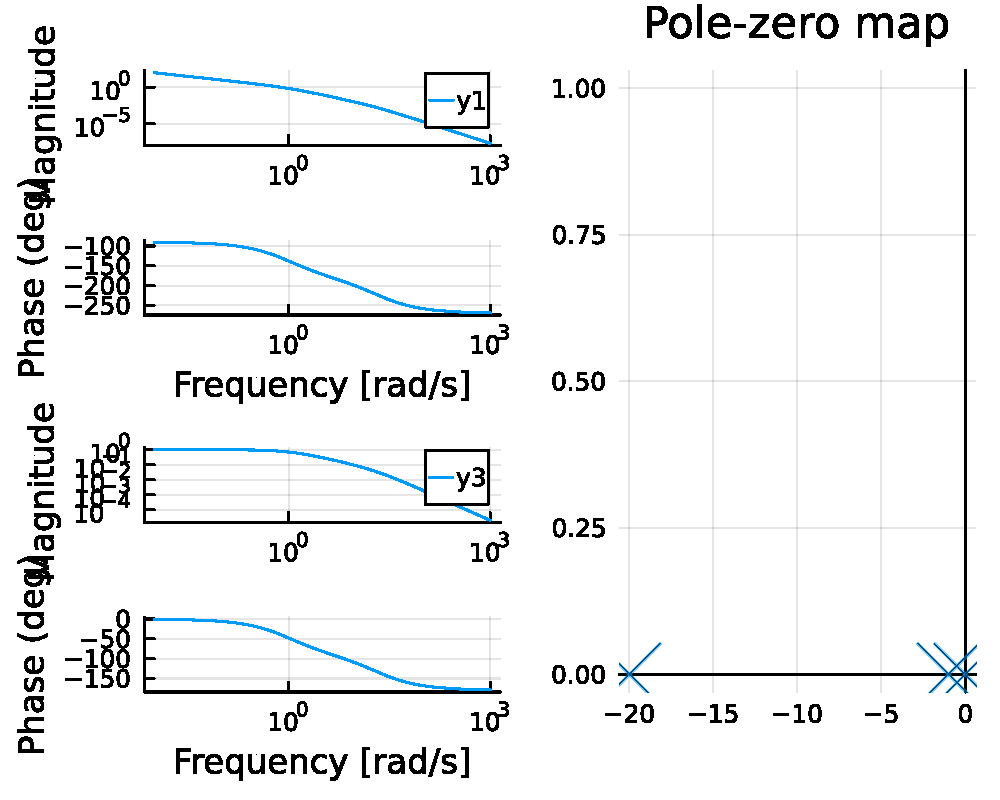
\includegraphics[keepaspectratio]{index_files/mediabag/block_on_slope/without_friction_files/figure-pdf/start-bode-output-1.pdf}}

}

\caption{Starting Bode Plot and PZ Map}

\end{figure}%

It has the shape we expect from a motor + friction. Slow pole for the
mass + friction and a faster pole for the current \& inductance.

Numerically they are:

\begin{Shaded}
\begin{Highlighting}[]
\FunctionTok{display}\NormalTok{(}\FunctionTok{eigvals}\NormalTok{(A))}
\end{Highlighting}
\end{Shaded}

\begin{verbatim}
3-element Vector{Float64}:
 -20.0
  -1.0
   0.0
\end{verbatim}

We see that we start with all the pole in the left-half plane, which is
good.

\section{Pole Placement}\label{pole-placement}

We can design a controller with pole placement.

For some reason pole placement doesn't work for the observer, I use a
Kalman Filter with random fast values.

\begin{Shaded}
\begin{Highlighting}[]
\FunctionTok{observability}\NormalTok{(A, C).isobservable }\OperatorTok{\&} 
\FunctionTok{controllability}\NormalTok{(A, B).iscontrollable; }\CommentTok{\#OK}

\NormalTok{ε }\OperatorTok{=} \FloatTok{0.01}\NormalTok{;}
\NormalTok{pp }\OperatorTok{=} \FloatTok{15.0}\NormalTok{;}
\NormalTok{poles\_cont }\OperatorTok{=} \OperatorTok{{-}}\FloatTok{2.0} \OperatorTok{*}\NormalTok{ [pp }\OperatorTok{+}\NormalTok{ ε, pp }\OperatorTok{{-}}\NormalTok{ ε, pp];}
\NormalTok{L }\OperatorTok{=} \FunctionTok{real}\NormalTok{(}\FunctionTok{place}\NormalTok{(sys, poles\_cont, }\OperatorTok{:}\NormalTok{c));}

\NormalTok{poles\_obs }\OperatorTok{=}\NormalTok{ poles\_cont }\OperatorTok{*} \FloatTok{10.0}\NormalTok{;}
\NormalTok{K }\OperatorTok{=} \FunctionTok{place}\NormalTok{(}\FloatTok{1.0} \OperatorTok{*}\NormalTok{ A}\OperatorTok{\textquotesingle{}}\NormalTok{, }\FloatTok{1.0} \OperatorTok{*}\NormalTok{ C}\OperatorTok{\textquotesingle{}}\NormalTok{, poles\_obs)}\CharTok{\textquotesingle{}}
\NormalTok{cont }\OperatorTok{=} \FunctionTok{observer\_controller}\NormalTok{(sys, L, K; direct}\OperatorTok{=}\ConstantTok{false}\NormalTok{);}
\end{Highlighting}
\end{Shaded}

We can check the effect of the new controller on the loop

\begin{Shaded}
\begin{Highlighting}[]
\NormalTok{closedLoop }\OperatorTok{=} \FunctionTok{feedback}\NormalTok{(sys }\OperatorTok{*}\NormalTok{ cont)}
\FunctionTok{print}\NormalTok{(}\FunctionTok{poles}\NormalTok{(closedLoop));}
\FunctionTok{setPlotScale}\NormalTok{(}\StringTok{"dB"}\NormalTok{)}
\FunctionTok{plot!}\NormalTok{(}\FunctionTok{bodeplot}\NormalTok{(closedLoop[}\FloatTok{1}\NormalTok{, }\FloatTok{1}\NormalTok{], }\FloatTok{0.1}\OperatorTok{:}\FloatTok{40}\NormalTok{), }\FunctionTok{pzmap}\NormalTok{(closedLoop))}
\end{Highlighting}
\end{Shaded}

\begin{verbatim}
ComplexF64[-29.979998924597755 + 0.0im, -30.000002152199972 + 0.0im, -30.019998923202337 + 0.0im, -300.0000000000004 + 0.0im, -300.1999999999752 + 0.0im, -299.80000000004117 + 0.0im]
\end{verbatim}

\pandocbounded{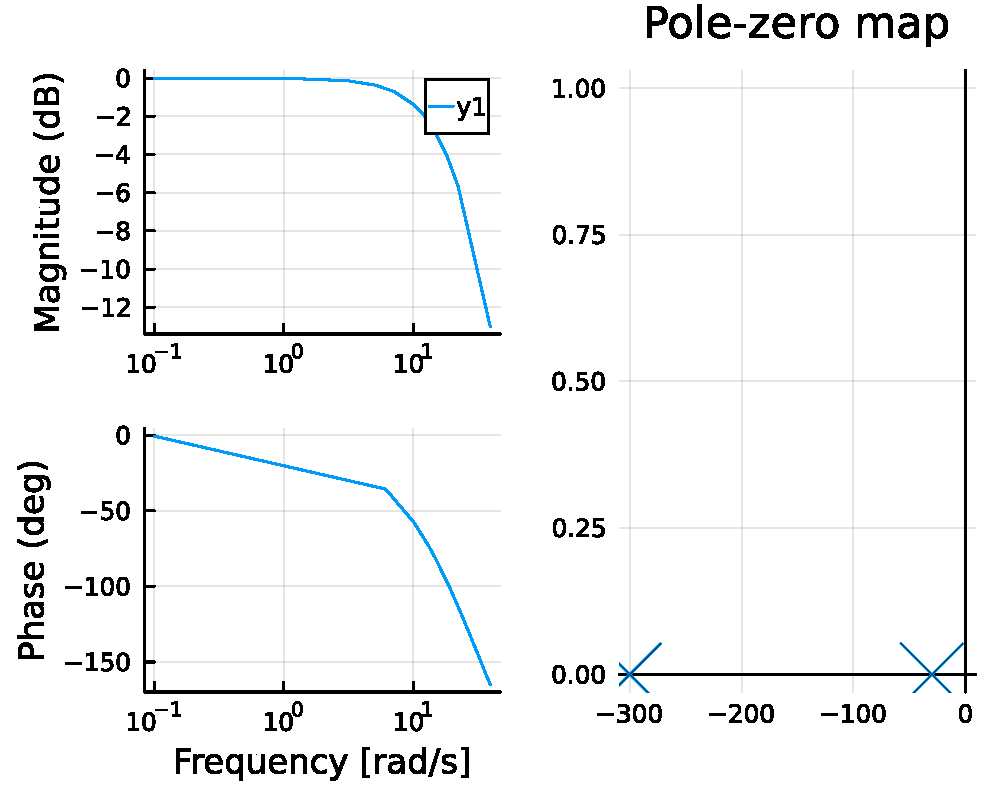
\includegraphics[keepaspectratio]{index_files/mediabag/block_on_slope/without_friction_files/figure-pdf/cell-5-output-2.pdf}}

We can compare this to the open-loop response in @start-bode. We can see
that we achieve unitary gain throughout the whole low-frequency range.

We can convert the pole placement controller into the standard PD gain
form.

\begin{Shaded}
\begin{Highlighting}[]
\NormalTok{K }\OperatorTok{=}\NormalTok{ L[}\FloatTok{1}\NormalTok{];}
\NormalTok{Ti }\OperatorTok{=} \FloatTok{0}\NormalTok{;}
\NormalTok{Td }\OperatorTok{=}\NormalTok{ L[}\FloatTok{2}\NormalTok{] }\OperatorTok{/}\NormalTok{ L[}\FloatTok{1}\NormalTok{];}
\NormalTok{pid }\OperatorTok{=} \FunctionTok{DiscretePID}\NormalTok{(; K, Ts, Ti, Td);}
\end{Highlighting}
\end{Shaded}

\section{Simulation}\label{simulation}

We can simulate this with a motor that only outputs the position:

\begin{Shaded}
\begin{Highlighting}[]
\NormalTok{sysreal }\OperatorTok{=} \FunctionTok{ss}\NormalTok{(A, B, [}\FloatTok{1} \FloatTok{0} \FloatTok{0}\NormalTok{], }\FloatTok{0.0}\NormalTok{)}
\NormalTok{ctrl }\OperatorTok{=} \KeywordTok{function}\NormalTok{ (x, t)}
\NormalTok{    y }\OperatorTok{=}\NormalTok{ (sysreal.C}\OperatorTok{*}\NormalTok{x)[] }\CommentTok{\# measurement}
\NormalTok{    d }\OperatorTok{=} \FloatTok{0} \OperatorTok{*}\NormalTok{ [}\FloatTok{1.0}\NormalTok{]        }\CommentTok{\# disturbance}
\NormalTok{    r }\OperatorTok{=} \FloatTok{2.0} \OperatorTok{*}\NormalTok{ (t }\OperatorTok{\textgreater{}=} \FloatTok{1}\NormalTok{) }\CommentTok{\# reference}
    \CommentTok{\# u = pid(r, y) \# control signal}
    \CommentTok{\# u + d \# Plant input is control signal + disturbance}
    \CommentTok{\# u =1}
    \ConstantTok{e} \OperatorTok{=}\NormalTok{ x }\OperatorTok{{-}}\NormalTok{ [r; }\FloatTok{0.0}\NormalTok{; }\FloatTok{0.0}\NormalTok{]}
    \ConstantTok{e}\NormalTok{[}\FloatTok{3}\NormalTok{] }\OperatorTok{=} \FloatTok{0.0} \CommentTok{\# torque not observable, just ignore it in the final feedback}
\NormalTok{    u }\OperatorTok{=} \OperatorTok{{-}}\NormalTok{L }\OperatorTok{*} \ConstantTok{e} \OperatorTok{+}\NormalTok{ d}
\NormalTok{    u }\OperatorTok{=}\NormalTok{ [}\FunctionTok{maximum}\NormalTok{([}\OperatorTok{{-}}\FloatTok{20.0} \FunctionTok{minimum}\NormalTok{([}\FloatTok{20.0}\NormalTok{ u])])]}
\KeywordTok{end}
\NormalTok{t }\OperatorTok{=} \FloatTok{0}\OperatorTok{:}\NormalTok{Ts}\OperatorTok{:}\NormalTok{Tf}

\NormalTok{res }\OperatorTok{=} \FunctionTok{lsim}\NormalTok{(sysreal, ctrl, t)}

\FunctionTok{display}\NormalTok{(}\FunctionTok{plot}\NormalTok{(res, }
\NormalTok{    plotu}\OperatorTok{=}\ConstantTok{true}\NormalTok{, }
\NormalTok{    plotx}\OperatorTok{=}\ConstantTok{true}\NormalTok{, }
\NormalTok{    ploty}\OperatorTok{=}\ConstantTok{false}
\NormalTok{    ))}
\FunctionTok{ylabel!}\NormalTok{(}\StringTok{"u"}\NormalTok{, sp}\OperatorTok{=}\FloatTok{1}\NormalTok{);}
\FunctionTok{ylabel!}\NormalTok{(}\StringTok{"x"}\NormalTok{, sp}\OperatorTok{=}\FloatTok{2}\NormalTok{);}
\FunctionTok{ylabel!}\NormalTok{(}\StringTok{"v"}\NormalTok{, sp}\OperatorTok{=}\FloatTok{3}\NormalTok{);}
\FunctionTok{ylabel!}\NormalTok{(}\StringTok{"T"}\NormalTok{, sp}\OperatorTok{=}\FloatTok{4}\NormalTok{);}
\end{Highlighting}
\end{Shaded}

\pandocbounded{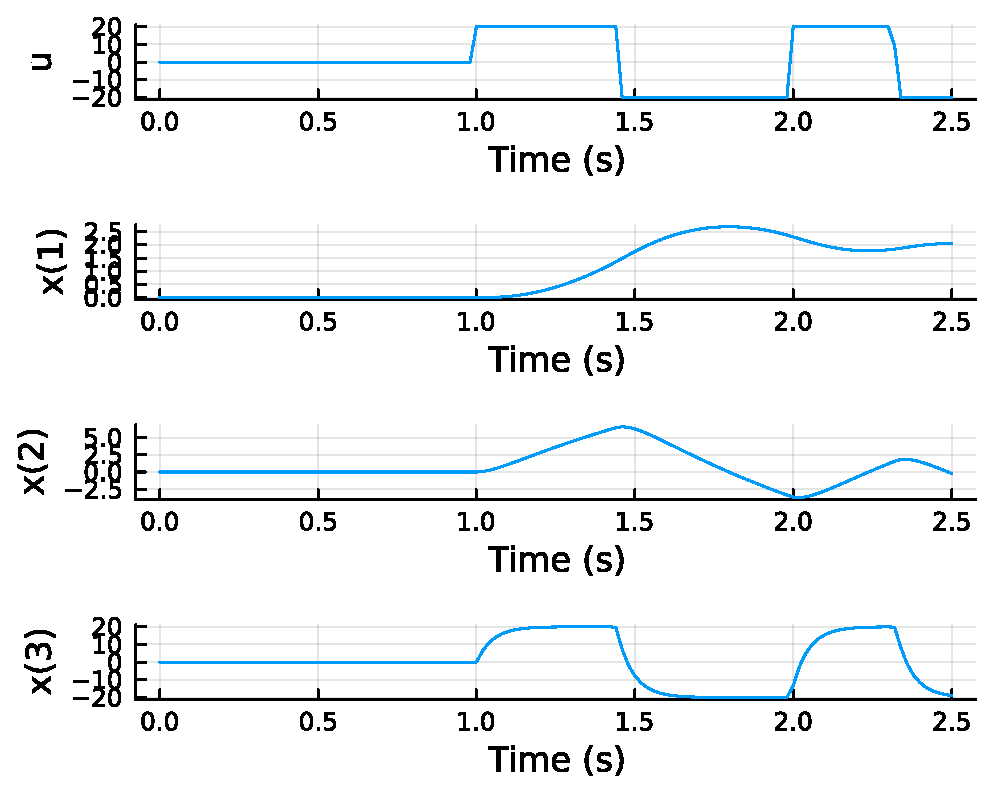
\includegraphics[keepaspectratio]{index_files/mediabag/block_on_slope/without_friction_files/figure-pdf/cell-7-output-1.pdf}}

For more stats:

\begin{Shaded}
\begin{Highlighting}[]
\NormalTok{si }\OperatorTok{=} \FunctionTok{stepinfo}\NormalTok{(res);}
\FunctionTok{plot}\NormalTok{(si);}\FunctionTok{title!}\NormalTok{(}\StringTok{"Step Response"}\NormalTok{)}
\end{Highlighting}
\end{Shaded}

\pandocbounded{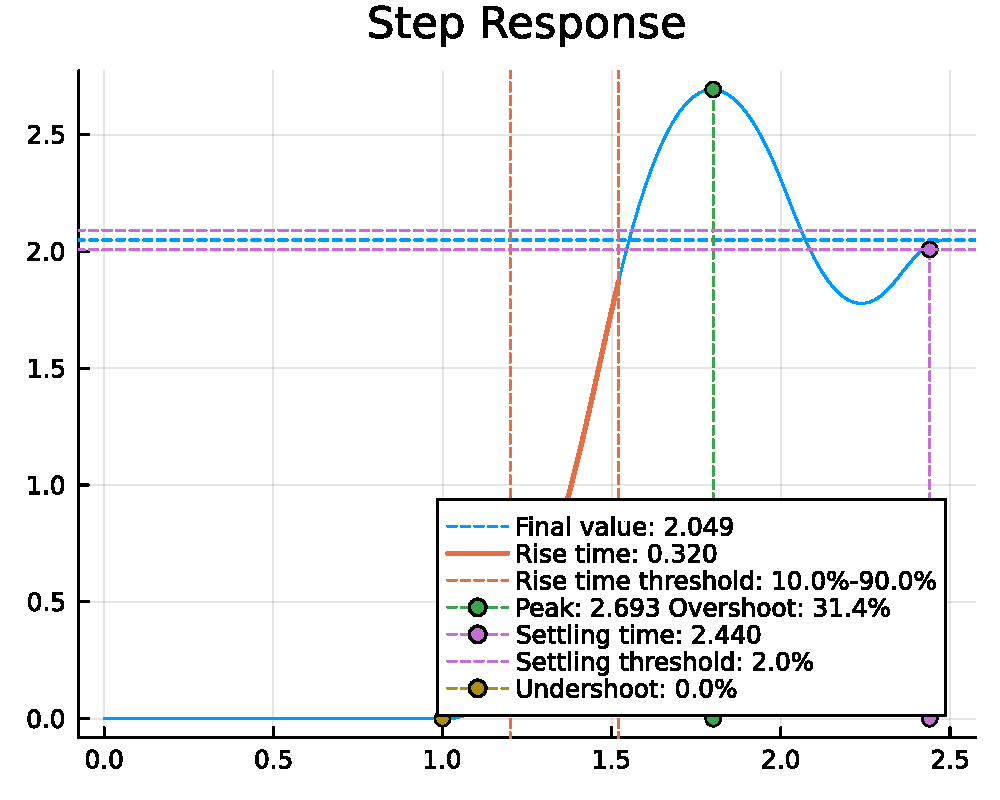
\includegraphics[keepaspectratio]{index_files/mediabag/block_on_slope/without_friction_files/figure-pdf/cell-8-output-1.pdf}}

We can also simulate it in a SIMULINK-like environment:

\begin{Shaded}
\begin{Highlighting}[]
\ImportTok{using} \BuiltInTok{FMI}\NormalTok{, }\BuiltInTok{DifferentialEquations}
\NormalTok{fmuPath }\OperatorTok{=} \FunctionTok{abspath}\NormalTok{(}\FunctionTok{joinpath}\NormalTok{(}\PreprocessorTok{@\_\_DIR\_\_}\NormalTok{,}
  \StringTok{".."}\NormalTok{,}\StringTok{".."}\NormalTok{,}
  \StringTok{"modelica"}\NormalTok{,}
  \StringTok{"ControlChallenges"}\NormalTok{,}
  \StringTok{"ControlChallenges.BlockOnSlope\_Challenges.Examples.WithFriction.fmu"}\NormalTok{))}
\NormalTok{fmu }\OperatorTok{=} \FunctionTok{loadFMU}\NormalTok{(fmuPath);}
\NormalTok{simData }\OperatorTok{=} \FunctionTok{simulateME}\NormalTok{(}
\NormalTok{    fmu,}
\NormalTok{    (}\FloatTok{0.0}\NormalTok{, }\FloatTok{5.0}\NormalTok{);}
\NormalTok{    recordValues}\OperatorTok{=}\NormalTok{[}\StringTok{"blockOnSlope.x"}\NormalTok{, }
    \StringTok{"blockOnSlope.xd"}\NormalTok{, }
    \StringTok{"blockOnSlope.usat"}\NormalTok{],}
\NormalTok{    showProgress}\OperatorTok{=}\ConstantTok{false}\NormalTok{);}
\FunctionTok{unloadFMU}\NormalTok{(fmu);}
\FunctionTok{plot}\NormalTok{(simData, states}\OperatorTok{=}\ConstantTok{false}\NormalTok{, timeEvents}\OperatorTok{=}\ConstantTok{false}\NormalTok{)}
\end{Highlighting}
\end{Shaded}

\pandocbounded{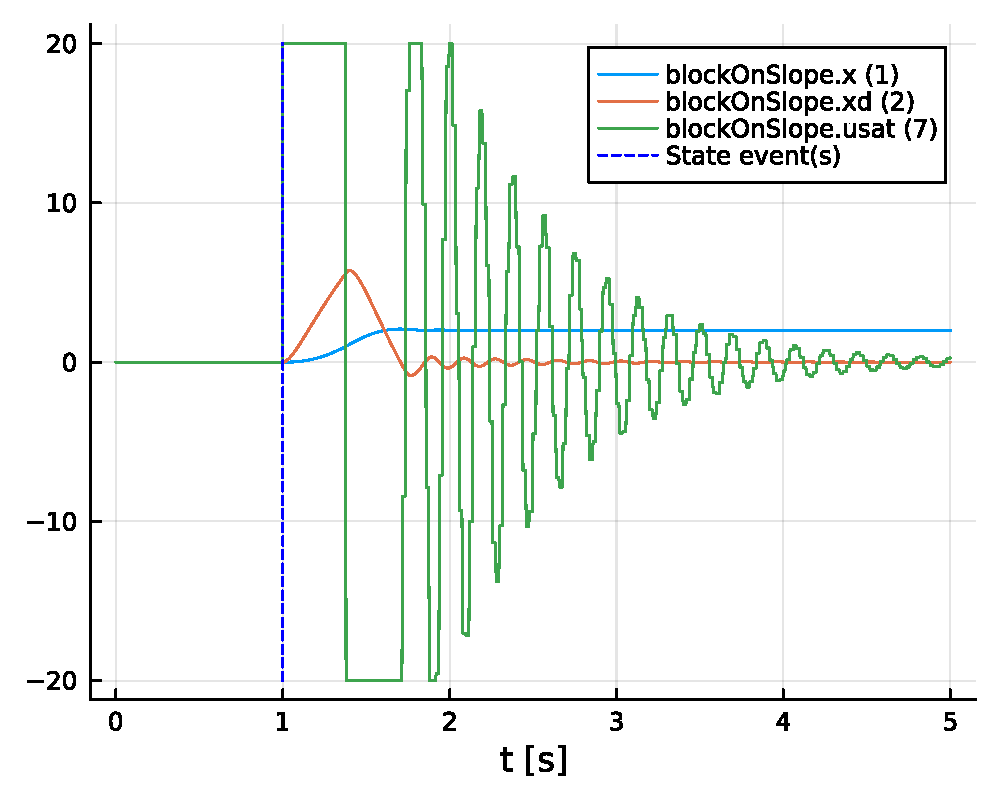
\includegraphics[keepaspectratio]{index_files/mediabag/block_on_slope/without_friction_files/figure-pdf/cell-9-output-1.pdf}}

There is a slight difference between the \texttt{lsim} simulation and
the FMU simulation. I need to recheck some stuff.



\chapter{Block With Friction}\label{block-with-friction}

Position Control with friction. Using Pole Placement + PD.

\hfill\break

\section{Response Analysis}\label{response-analysis}

\begin{Shaded}
\begin{Highlighting}[]
\ImportTok{using} \BuiltInTok{CCS}
\ImportTok{using} \BuiltInTok{ControlSystems}\NormalTok{, }\BuiltInTok{Plots}\NormalTok{, }\BuiltInTok{LinearAlgebra}\NormalTok{, }\BuiltInTok{RobustAndOptimalControl}
\NormalTok{CCS.}\FunctionTok{setupEnv}\NormalTok{()}

\NormalTok{contSys }\OperatorTok{=}\NormalTok{ CCS.blockModel.}\FunctionTok{csys}\NormalTok{(;g }\OperatorTok{=} \FloatTok{0}\NormalTok{, α }\OperatorTok{=} \FloatTok{0}\NormalTok{ , μ }\OperatorTok{=} \FloatTok{1}\NormalTok{, τ }\OperatorTok{=}\FloatTok{20}\NormalTok{)}
\FunctionTok{plot!}\NormalTok{(}\FunctionTok{bodeplot}\NormalTok{(contSys[}\FloatTok{1}\NormalTok{,}\FloatTok{1}\NormalTok{]),}\FunctionTok{pzmap}\NormalTok{(contSys))}
\end{Highlighting}
\end{Shaded}

\begin{verbatim}
Precompiling CCS...
  12450.0 ms  ✓ CCS
  1 dependency successfully precompiled in 16 seconds. 510 already precompiled.
\end{verbatim}

\begin{figure}[H]

{\centering \pandocbounded{\includegraphics[keepaspectratio]{index_files/mediabag/block_on_slope/with_friction_files/figure-pdf/start-bode-output-2.pdf}}

}

\caption{Starting Bode Plot and Pole/Zero Map}

\end{figure}%

It has the shape we expect from a motor + friction. Slow pole for the
mass + friction and a faster pole for the current \& inductance.

Numerically they are:

\begin{Shaded}
\begin{Highlighting}[]
\FunctionTok{display}\NormalTok{(}\FunctionTok{eigvals}\NormalTok{(contSys.A))}
\end{Highlighting}
\end{Shaded}

\begin{verbatim}
3-element Vector{Float64}:
 -20.0
  -1.0
   0.0
\end{verbatim}

We see that we start with all the poles in the left-half plane, which is
good.

\section{Pole Placement}\label{pole-placement-1}

We can design a controller with pole placement.

For some reason pole placement doesn't work for the observer, I use a
Kalman Filter with random fast values.

\begin{Shaded}
\begin{Highlighting}[]
\FunctionTok{observability}\NormalTok{(contSys.A,contSys.C).isobservable }\OperatorTok{||} \FunctionTok{error}\NormalTok{(}\StringTok{"System is not observable"}\NormalTok{)}
\FunctionTok{controllability}\NormalTok{(contSys.A,contSys.B).iscontrollable }\OperatorTok{||} \FunctionTok{error}\NormalTok{(}\StringTok{"System is not controllable"}\NormalTok{)}

\NormalTok{ε }\OperatorTok{=} \FloatTok{0.01}\NormalTok{;}
\NormalTok{pp }\OperatorTok{=} \FloatTok{15.0}\NormalTok{;}
\NormalTok{poles\_cont }\OperatorTok{=} \OperatorTok{{-}}\NormalTok{ [pp }\OperatorTok{+}\NormalTok{ ε, pp }\OperatorTok{{-}}\NormalTok{ ε, pp];}
\NormalTok{L }\OperatorTok{=} \FunctionTok{real}\NormalTok{(}\FunctionTok{place}\NormalTok{(contSys, poles\_cont, }\OperatorTok{:}\NormalTok{c));}


\NormalTok{poles\_obs }\OperatorTok{=}\NormalTok{ poles\_cont }\OperatorTok{*} \FloatTok{10.0}\NormalTok{;}
\NormalTok{K }\OperatorTok{=} \FunctionTok{place}\NormalTok{(contSys, poles\_obs, }\OperatorTok{:}\NormalTok{o)}
\NormalTok{obs\_controller }\OperatorTok{=} \FunctionTok{observer\_controller}\NormalTok{(contSys, L, K; direct}\OperatorTok{=}\ConstantTok{false}\NormalTok{);}
\NormalTok{fsf\_controller }\OperatorTok{=} \FunctionTok{named\_ss}\NormalTok{(obs\_controller, u }\OperatorTok{=}\NormalTok{ [}\OperatorTok{:}\NormalTok{ref\_S, }\OperatorTok{:}\NormalTok{ref\_V], y }\OperatorTok{=}\NormalTok{ [}\OperatorTok{:}\NormalTok{u]);}
\end{Highlighting}
\end{Shaded}

We can check the effect of the new controller on the loop

\begin{Shaded}
\begin{Highlighting}[]
\NormalTok{closedLoop }\OperatorTok{=} \FunctionTok{feedback}\NormalTok{( contSys }\OperatorTok{*}\NormalTok{ fsf\_controller);}
\FunctionTok{print}\NormalTok{(}\FunctionTok{poles}\NormalTok{(closedLoop));}
\FunctionTok{setPlotScale}\NormalTok{(}\StringTok{"dB"}\NormalTok{)}
\FunctionTok{plot!}\NormalTok{(}\FunctionTok{bodeplot}\NormalTok{(closedLoop[}\FloatTok{1}\NormalTok{,}\FloatTok{1}\NormalTok{], }\FloatTok{0.1}\OperatorTok{:}\FloatTok{40}\NormalTok{), }\FunctionTok{pzmap}\NormalTok{(closedLoop))}
\end{Highlighting}
\end{Shaded}

\begin{verbatim}
ComplexF64[-14.990000366343788 + 0.0im, -14.999999266673722 + 0.0im, -15.010000366982666 + 0.0im, -149.99999999999986 + 0.0im, -150.10000000002432 + 0.0im, -149.8999999999607 + 0.0im]
\end{verbatim}

\pandocbounded{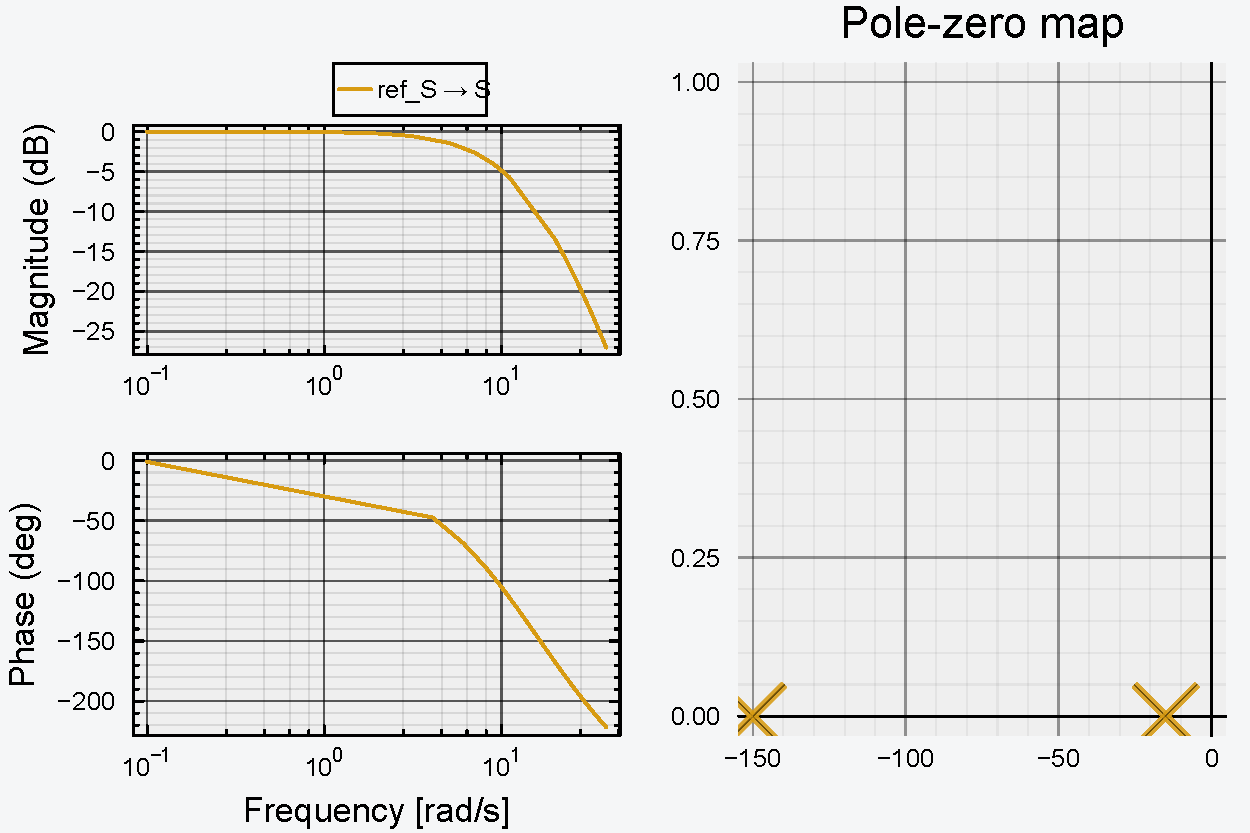
\includegraphics[keepaspectratio]{index_files/mediabag/block_on_slope/with_friction_files/figure-pdf/cell-5-output-2.pdf}}

We can compare this to the open-loop response in @start-bode. We can see
that we achieve unitary gain throughout the whole low-frequency range.

We can convert the pole placement controller into the standard PD gain
form.

\begin{Shaded}
\begin{Highlighting}[]
\ImportTok{using} \BuiltInTok{DiscretePIDs}
\NormalTok{Ts }\OperatorTok{=} \FloatTok{0.02} \CommentTok{\# sampling time}
\NormalTok{Tf }\OperatorTok{=} \FloatTok{2.5}\NormalTok{; }\CommentTok{\#final simulation time}

\NormalTok{K }\OperatorTok{=}\NormalTok{ L[}\FloatTok{1}\NormalTok{];}
\NormalTok{Ti }\OperatorTok{=} \FloatTok{0}\NormalTok{;}
\NormalTok{Td }\OperatorTok{=}\NormalTok{ L[}\FloatTok{2}\NormalTok{] }\OperatorTok{/}\NormalTok{ L[}\FloatTok{1}\NormalTok{];}

\NormalTok{pid }\OperatorTok{=} \FunctionTok{DiscretePID}\NormalTok{(; K, Ts, Ti, Td);}
\end{Highlighting}
\end{Shaded}

\section{Simulation}\label{simulation-1}

We can simulate this with a motor that only outputs the position:

\begin{Shaded}
\begin{Highlighting}[]
\NormalTok{sysreal }\OperatorTok{=} \FunctionTok{ss}\NormalTok{(contSys.A, contSys.B, [}\FloatTok{1} \FloatTok{0} \FloatTok{0}\NormalTok{], }\FloatTok{0.0}\NormalTok{)}
\NormalTok{ctrl }\OperatorTok{=} \KeywordTok{function}\NormalTok{ (x, t)}
\NormalTok{    y }\OperatorTok{=}\NormalTok{ (sysreal.C}\OperatorTok{*}\NormalTok{x)[] }\CommentTok{\# measurement}
\NormalTok{    d }\OperatorTok{=} \FloatTok{0} \OperatorTok{*}\NormalTok{ [}\FloatTok{1.0}\NormalTok{]        }\CommentTok{\# disturbance}
\NormalTok{    r }\OperatorTok{=} \FloatTok{2.0} \OperatorTok{*}\NormalTok{ (t }\OperatorTok{\textgreater{}=} \FloatTok{1}\NormalTok{) }\CommentTok{\# reference}
    \CommentTok{\# u = pid(r, y) \# control signal}
    \CommentTok{\# u + d \# Plant input is control signal + disturbance}
    \CommentTok{\# u =1}
    \ConstantTok{e} \OperatorTok{=}\NormalTok{ x }\OperatorTok{{-}}\NormalTok{ [r; }\FloatTok{0.0}\NormalTok{; }\FloatTok{0.0}\NormalTok{]}
    \ConstantTok{e}\NormalTok{[}\FloatTok{3}\NormalTok{] }\OperatorTok{=} \FloatTok{0.0} \CommentTok{\# torque not observable, just ignore it in the final feedback}
\NormalTok{    u }\OperatorTok{=} \OperatorTok{{-}}\NormalTok{L }\OperatorTok{*} \ConstantTok{e} \OperatorTok{+}\NormalTok{ d}
\NormalTok{    u }\OperatorTok{=}\NormalTok{ [}\FunctionTok{maximum}\NormalTok{([}\OperatorTok{{-}}\FloatTok{20.0} \FunctionTok{minimum}\NormalTok{([}\FloatTok{20.0}\NormalTok{ u])])]}
\KeywordTok{end}
\NormalTok{t }\OperatorTok{=} \FloatTok{0}\OperatorTok{:}\NormalTok{Ts}\OperatorTok{:}\NormalTok{Tf}

\NormalTok{res }\OperatorTok{=} \FunctionTok{lsim}\NormalTok{(sysreal, ctrl, t)}

\FunctionTok{display}\NormalTok{(}\FunctionTok{plot}\NormalTok{(res, }
\NormalTok{    plotu}\OperatorTok{=}\ConstantTok{true}\NormalTok{, }
\NormalTok{    plotx}\OperatorTok{=}\ConstantTok{true}\NormalTok{, }
\NormalTok{    ploty}\OperatorTok{=}\ConstantTok{false}
\NormalTok{    ))}
\FunctionTok{ylabel!}\NormalTok{(}\StringTok{"u"}\NormalTok{, sp}\OperatorTok{=}\FloatTok{1}\NormalTok{);}
\FunctionTok{ylabel!}\NormalTok{(}\StringTok{"x"}\NormalTok{, sp}\OperatorTok{=}\FloatTok{2}\NormalTok{);}
\FunctionTok{ylabel!}\NormalTok{(}\StringTok{"v"}\NormalTok{, sp}\OperatorTok{=}\FloatTok{3}\NormalTok{);}
\FunctionTok{ylabel!}\NormalTok{(}\StringTok{"T"}\NormalTok{, sp}\OperatorTok{=}\FloatTok{4}\NormalTok{);}
\end{Highlighting}
\end{Shaded}

\pandocbounded{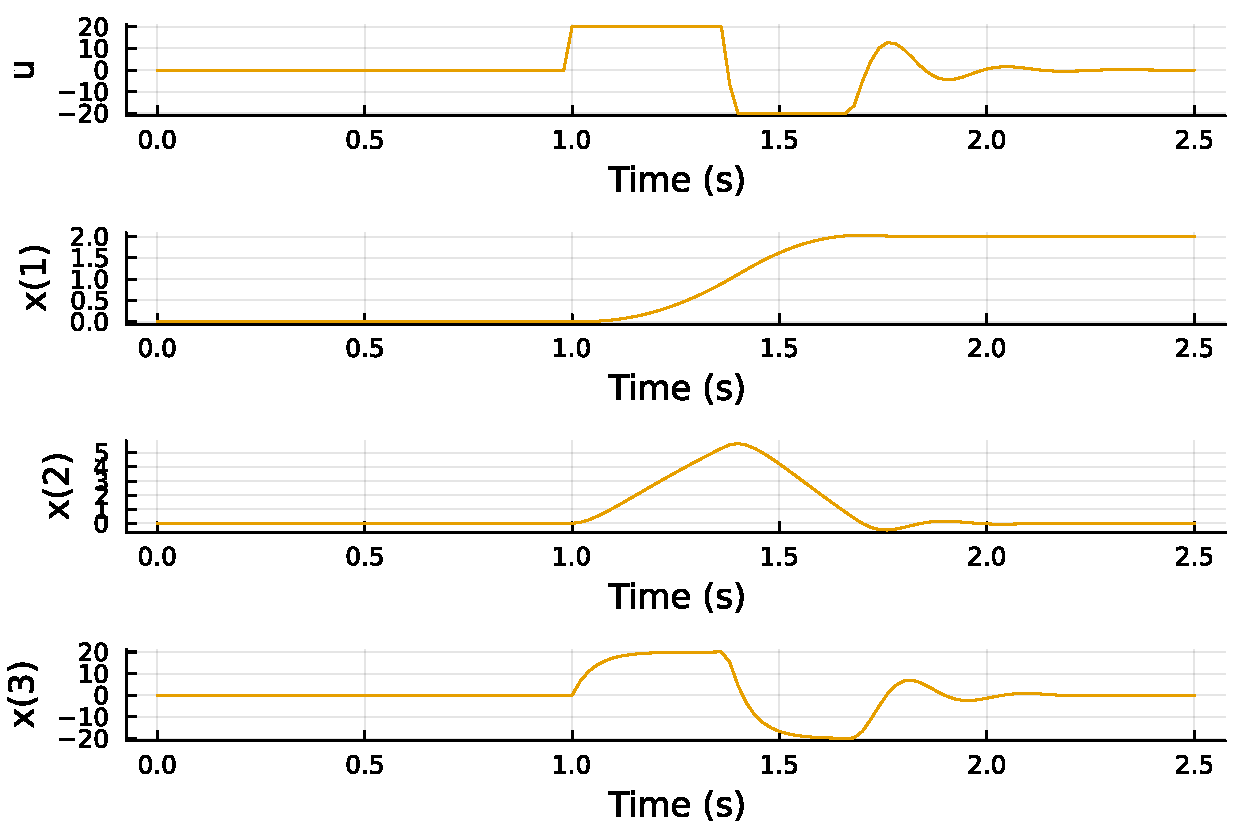
\includegraphics[keepaspectratio]{index_files/mediabag/block_on_slope/with_friction_files/figure-pdf/cell-7-output-1.pdf}}

For more stats:

\begin{Shaded}
\begin{Highlighting}[]
\NormalTok{si }\OperatorTok{=} \FunctionTok{stepinfo}\NormalTok{(res);}
\FunctionTok{plot}\NormalTok{(si);}\FunctionTok{title!}\NormalTok{(}\StringTok{"Step Response"}\NormalTok{)}
\end{Highlighting}
\end{Shaded}

\pandocbounded{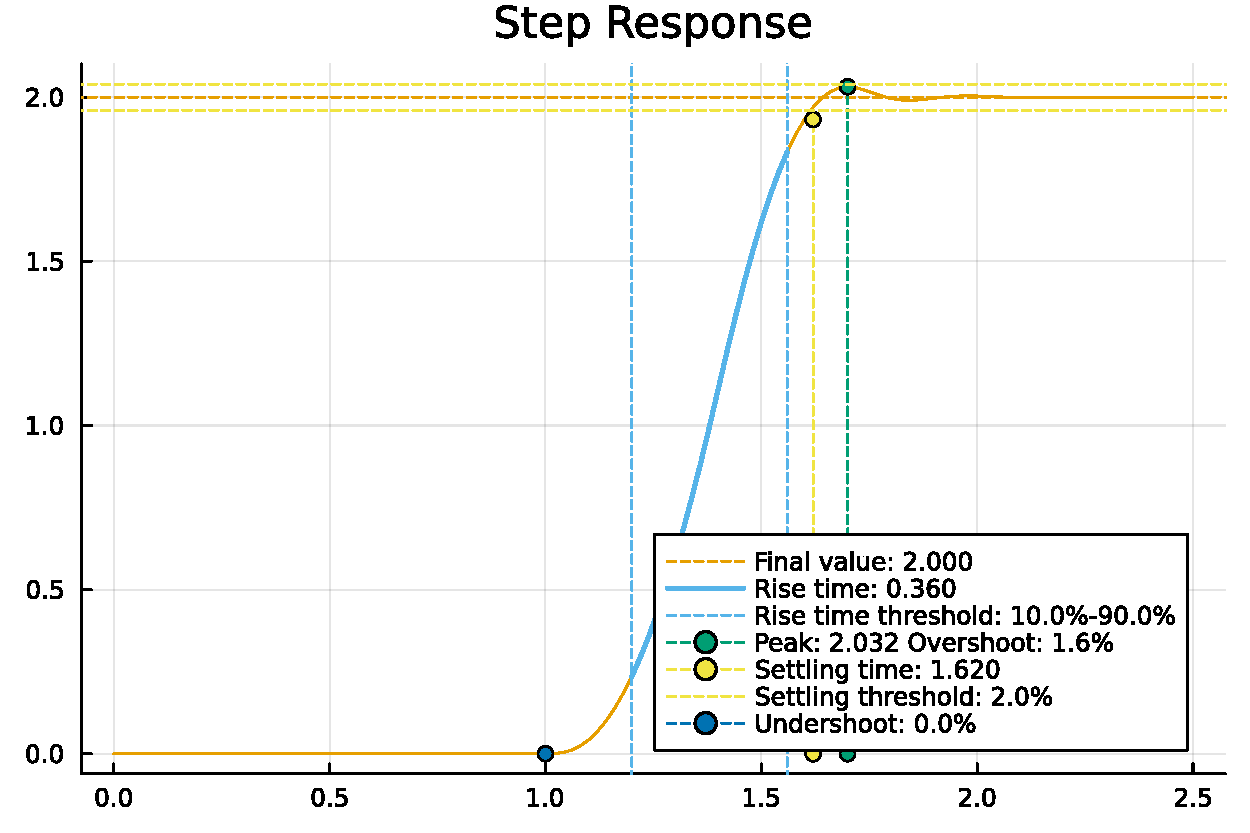
\includegraphics[keepaspectratio]{index_files/mediabag/block_on_slope/with_friction_files/figure-pdf/cell-8-output-1.pdf}}

We can also simulate it in a SIMULINK-like environment:

\begin{Shaded}
\begin{Highlighting}[]
\ImportTok{using} \BuiltInTok{FMI}\NormalTok{, }\BuiltInTok{DifferentialEquations}
\NormalTok{fmuPath }\OperatorTok{=} \FunctionTok{abspath}\NormalTok{(}\FunctionTok{joinpath}\NormalTok{(}\PreprocessorTok{@\_\_DIR\_\_}\NormalTok{,}
  \StringTok{".."}\NormalTok{,}\StringTok{".."}\NormalTok{,}
  \StringTok{"modelica"}\NormalTok{,}
  \StringTok{"ControlChallenges"}\NormalTok{,}
  \StringTok{"ControlChallenges.BlockOnSlope\_Challenges.Examples.WithFriction.fmu"}\NormalTok{))}
\NormalTok{fmu }\OperatorTok{=} \FunctionTok{loadFMU}\NormalTok{(fmuPath);}
\NormalTok{simData }\OperatorTok{=} \FunctionTok{simulateME}\NormalTok{(}
\NormalTok{    fmu,}
\NormalTok{    (}\FloatTok{0.0}\NormalTok{, }\FloatTok{5.0}\NormalTok{);}
\NormalTok{    recordValues}\OperatorTok{=}\NormalTok{[}\StringTok{"blockOnSlope.x"}\NormalTok{, }
    \StringTok{"blockOnSlope.xd"}\NormalTok{, }
    \StringTok{"blockOnSlope.usat"}\NormalTok{],}
\NormalTok{    showProgress}\OperatorTok{=}\ConstantTok{false}\NormalTok{);}
\FunctionTok{unloadFMU}\NormalTok{(fmu);}
\FunctionTok{plot}\NormalTok{(simData, states}\OperatorTok{=}\ConstantTok{false}\NormalTok{, timeEvents}\OperatorTok{=}\ConstantTok{false}\NormalTok{)}
\end{Highlighting}
\end{Shaded}

\pandocbounded{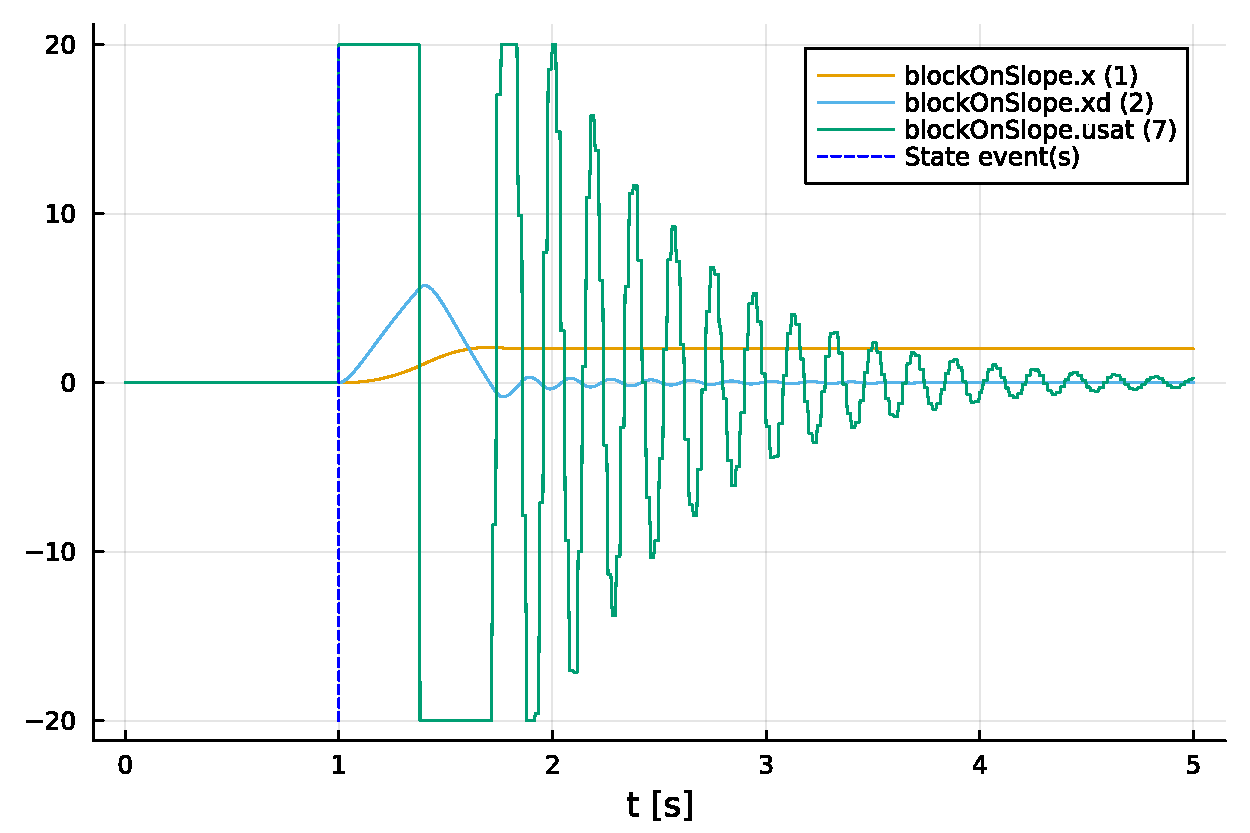
\includegraphics[keepaspectratio]{index_files/mediabag/block_on_slope/with_friction_files/figure-pdf/cell-9-output-1.pdf}}

There is a slight difference between the \texttt{lsim} simulation and
the FMU simulation. I need to recheck some stuff.



\chapter{Block on a slope}\label{block-on-a-slope-1}

Position Control with friction. Using Pole Placement + PD.

\hfill\break

\section{Response Analysis}\label{response-analysis-1}

\begin{Shaded}
\begin{Highlighting}[]
\ImportTok{using} \BuiltInTok{CCS}
\ImportTok{using} \BuiltInTok{ControlSystems}\NormalTok{, }\BuiltInTok{Plots}\NormalTok{, }\BuiltInTok{LinearAlgebra}\NormalTok{, }\BuiltInTok{RobustAndOptimalControl}
\NormalTok{CCS.}\FunctionTok{setupEnv}\NormalTok{()}

\NormalTok{contSys }\OperatorTok{=}\NormalTok{ CCS.blockModel.}\FunctionTok{csys}\NormalTok{(;g }\OperatorTok{=} \FloatTok{0}\NormalTok{, α }\OperatorTok{=} \FloatTok{0}\NormalTok{ , μ }\OperatorTok{=} \FloatTok{1}\NormalTok{, τ }\OperatorTok{=}\FloatTok{20.0}\NormalTok{)}
\FunctionTok{plot!}\NormalTok{(}\FunctionTok{bodeplot}\NormalTok{(contSys[}\FloatTok{1}\NormalTok{,}\FloatTok{1}\NormalTok{]),}\FunctionTok{pzmap}\NormalTok{(contSys))}
\end{Highlighting}
\end{Shaded}

\begin{verbatim}
Precompiling CCS...
  12287.4 ms  ✓ CCS
  1 dependency successfully precompiled in 15 seconds. 510 already precompiled.
\end{verbatim}

\begin{figure}[H]

{\centering \pandocbounded{\includegraphics[keepaspectratio]{index_files/mediabag/block_on_slope/slope_files/figure-pdf/start-bode-output-2.pdf}}

}

\caption{Starting Bode Plot and PZ Map}

\end{figure}%

It has the shape we expect from a motor + friction. Slow pole for the
mass + friction and a faster pole for the current \& inductance.

Numerically they are:

\begin{Shaded}
\begin{Highlighting}[]
\FunctionTok{display}\NormalTok{(}\FunctionTok{eigvals}\NormalTok{(contSys.A))}
\end{Highlighting}
\end{Shaded}

\begin{verbatim}
3-element Vector{Float64}:
 -20.0
  -1.0
   0.0
\end{verbatim}

We see that we start with all the poles in the left-half plane, which is
good.

\section{Pole Placement}\label{pole-placement-2}

We can design a controller with pole placement.

For some reason pole placement doesn't work for the observer, I use a
Kalman Filter with random fast values.

\begin{Shaded}
\begin{Highlighting}[]
\FunctionTok{observability}\NormalTok{(contSys.A,contSys.C).isobservable }\OperatorTok{||} \FunctionTok{error}\NormalTok{(}\StringTok{"System is not observable"}\NormalTok{)}
\FunctionTok{controllability}\NormalTok{(contSys.A,contSys.B).iscontrollable }\OperatorTok{||} \FunctionTok{error}\NormalTok{(}\StringTok{"System is not controllable"}\NormalTok{)}

\NormalTok{ε }\OperatorTok{=} \FloatTok{0.01}\NormalTok{;}
\NormalTok{pp }\OperatorTok{=} \FloatTok{15.0}\NormalTok{;}
\NormalTok{poles\_cont }\OperatorTok{=} \OperatorTok{{-}}\NormalTok{ [pp }\OperatorTok{+}\NormalTok{ ε, pp }\OperatorTok{{-}}\NormalTok{ ε, pp];}
\NormalTok{L }\OperatorTok{=} \FunctionTok{real}\NormalTok{(}\FunctionTok{place}\NormalTok{(contSys, poles\_cont, }\OperatorTok{:}\NormalTok{c));}


\NormalTok{poles\_obs }\OperatorTok{=}\NormalTok{ poles\_cont }\OperatorTok{*} \FloatTok{10.0}\NormalTok{;}
\NormalTok{K }\OperatorTok{=} \FunctionTok{place}\NormalTok{(contSys, poles\_obs, }\OperatorTok{:}\NormalTok{o)}
\NormalTok{obs\_controller }\OperatorTok{=} \FunctionTok{observer\_controller}\NormalTok{(contSys, L, K; direct}\OperatorTok{=}\ConstantTok{false}\NormalTok{);}
\NormalTok{fsf\_controller }\OperatorTok{=} \FunctionTok{named\_ss}\NormalTok{(obs\_controller, u }\OperatorTok{=}\NormalTok{ [}\OperatorTok{:}\NormalTok{ref\_S, }\OperatorTok{:}\NormalTok{ref\_V], y }\OperatorTok{=}\NormalTok{ [}\OperatorTok{:}\NormalTok{u])}
\end{Highlighting}
\end{Shaded}

\begin{verbatim}
NamedStateSpace{Continuous, Float64}
A = 
  -150.0                         8.033684828490095e-12    0.0
     1.0915557686859107e-5    -279.9999999999851          1.0
 -3374.9970813429577        -17530.98989999806          -44.0
B = 
 150.0                        0.9999999999919663
  -1.0915557686859107e-5    278.9999999999851
  -0.0014186570429435138  16899.989999998063
C = 
 168.74992500000002  31.549995000000003  1.2000000000000002
D = 
 0.0  0.0

Continuous-time state-space model
With state  names: x1 x2 x3
     input  names: ref_S ref_V
     output names: u
\end{verbatim}

We can check the effect of the new controller on the loop

\begin{Shaded}
\begin{Highlighting}[]
\NormalTok{closedLoop }\OperatorTok{=} \FunctionTok{feedback}\NormalTok{( contSys }\OperatorTok{*}\NormalTok{ fsf\_controller);}
\FunctionTok{print}\NormalTok{(}\FunctionTok{poles}\NormalTok{(closedLoop));}
\FunctionTok{setPlotScale}\NormalTok{(}\StringTok{"dB"}\NormalTok{)}
\FunctionTok{plot!}\NormalTok{(}\FunctionTok{bodeplot}\NormalTok{(closedLoop[}\FloatTok{1}\NormalTok{,}\FloatTok{1}\NormalTok{], }\FloatTok{0.1}\OperatorTok{:}\FloatTok{40}\NormalTok{), }\FunctionTok{pzmap}\NormalTok{(closedLoop))}
\end{Highlighting}
\end{Shaded}

\begin{verbatim}
ComplexF64[-14.990000366343788 + 0.0im, -14.999999266673722 + 0.0im, -15.010000366982666 + 0.0im, -149.99999999999986 + 0.0im, -150.10000000002432 + 0.0im, -149.8999999999607 + 0.0im]
\end{verbatim}

\pandocbounded{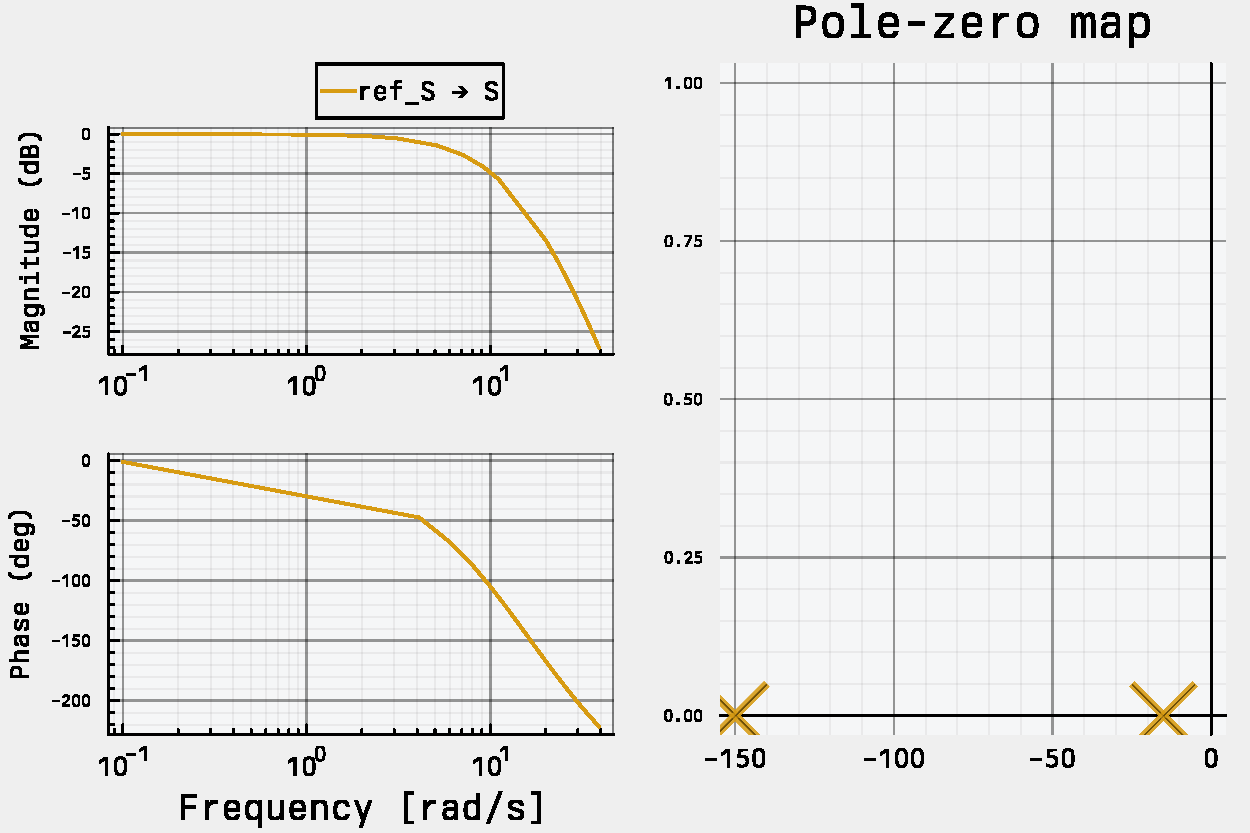
\includegraphics[keepaspectratio]{index_files/mediabag/block_on_slope/slope_files/figure-pdf/cell-5-output-2.pdf}}

We can compare this to the open-loop response in @start-bode. We can see
that we achieve unitary gain throughout the whole low-frequency range.

We can convert the pole placement controller into the standard PD gain
form.

\begin{Shaded}
\begin{Highlighting}[]
\ImportTok{using} \BuiltInTok{DiscretePIDs}
\NormalTok{Ts }\OperatorTok{=} \FloatTok{0.02} \CommentTok{\# sampling time}
\NormalTok{Tf }\OperatorTok{=} \FloatTok{2.5}\NormalTok{; }\CommentTok{\#final simulation time}

\NormalTok{K }\OperatorTok{=}\NormalTok{ L[}\FloatTok{1}\NormalTok{];}
\NormalTok{Ti }\OperatorTok{=} \FloatTok{0}\NormalTok{;}
\NormalTok{Td }\OperatorTok{=}\NormalTok{ L[}\FloatTok{2}\NormalTok{] }\OperatorTok{/}\NormalTok{ L[}\FloatTok{1}\NormalTok{];}

\NormalTok{pid }\OperatorTok{=} \FunctionTok{DiscretePID}\NormalTok{(; K, Ts, Ti, Td);}
\end{Highlighting}
\end{Shaded}

\section{Simulation}\label{simulation-2}

We can simulate this with a motor that only outputs the position:

\begin{Shaded}
\begin{Highlighting}[]
\NormalTok{sysreal }\OperatorTok{=} \FunctionTok{ss}\NormalTok{(contSys.A, contSys.B, [}\FloatTok{1} \FloatTok{0} \FloatTok{0}\NormalTok{], }\FloatTok{0.0}\NormalTok{)}
\NormalTok{ctrl }\OperatorTok{=} \KeywordTok{function}\NormalTok{ (x, t)}
\NormalTok{    y }\OperatorTok{=}\NormalTok{ (sysreal.C}\OperatorTok{*}\NormalTok{x)[] }\CommentTok{\# measurement}
\NormalTok{    d }\OperatorTok{=} \FloatTok{0} \OperatorTok{*}\NormalTok{ [}\FloatTok{1.0}\NormalTok{]        }\CommentTok{\# disturbance}
\NormalTok{    r }\OperatorTok{=} \FloatTok{2.0} \OperatorTok{*}\NormalTok{ (t }\OperatorTok{\textgreater{}=} \FloatTok{1}\NormalTok{) }\CommentTok{\# reference}
    \CommentTok{\# u = pid(r, y) \# control signal}
    \CommentTok{\# u + d \# Plant input is control signal + disturbance}
    \CommentTok{\# u =1}
    \ConstantTok{e} \OperatorTok{=}\NormalTok{ x }\OperatorTok{{-}}\NormalTok{ [r; }\FloatTok{0.0}\NormalTok{; }\FloatTok{0.0}\NormalTok{]}
    \ConstantTok{e}\NormalTok{[}\FloatTok{3}\NormalTok{] }\OperatorTok{=} \FloatTok{0.0} \CommentTok{\# torque not observable, just ignore it in the final feedback}
\NormalTok{    u }\OperatorTok{=} \OperatorTok{{-}}\NormalTok{L }\OperatorTok{*} \ConstantTok{e} \OperatorTok{+}\NormalTok{ d}
\NormalTok{    u }\OperatorTok{=}\NormalTok{ [}\FunctionTok{maximum}\NormalTok{([}\OperatorTok{{-}}\FloatTok{20.0} \FunctionTok{minimum}\NormalTok{([}\FloatTok{20.0}\NormalTok{ u])])]}
\KeywordTok{end}
\NormalTok{t }\OperatorTok{=} \FloatTok{0}\OperatorTok{:}\NormalTok{Ts}\OperatorTok{:}\NormalTok{Tf}

\NormalTok{res }\OperatorTok{=} \FunctionTok{lsim}\NormalTok{(sysreal, ctrl, t)}

\FunctionTok{display}\NormalTok{(}\FunctionTok{plot}\NormalTok{(res, }
\NormalTok{    plotu}\OperatorTok{=}\ConstantTok{true}\NormalTok{, }
\NormalTok{    plotx}\OperatorTok{=}\ConstantTok{true}\NormalTok{, }
\NormalTok{    ploty}\OperatorTok{=}\ConstantTok{false}
\NormalTok{    ));}\FunctionTok{ylabel!}\NormalTok{(}\StringTok{"u"}\NormalTok{, sp}\OperatorTok{=}\FloatTok{1}\NormalTok{);}\FunctionTok{ylabel!}\NormalTok{(}\StringTok{"x"}\NormalTok{, sp}\OperatorTok{=}\FloatTok{2}\NormalTok{);}\FunctionTok{ylabel!}\NormalTok{(}\StringTok{"v"}\NormalTok{, sp}\OperatorTok{=}\FloatTok{3}\NormalTok{);}\FunctionTok{ylabel!}\NormalTok{(}\StringTok{"T"}\NormalTok{, sp}\OperatorTok{=}\FloatTok{4}\NormalTok{);}
\end{Highlighting}
\end{Shaded}

\pandocbounded{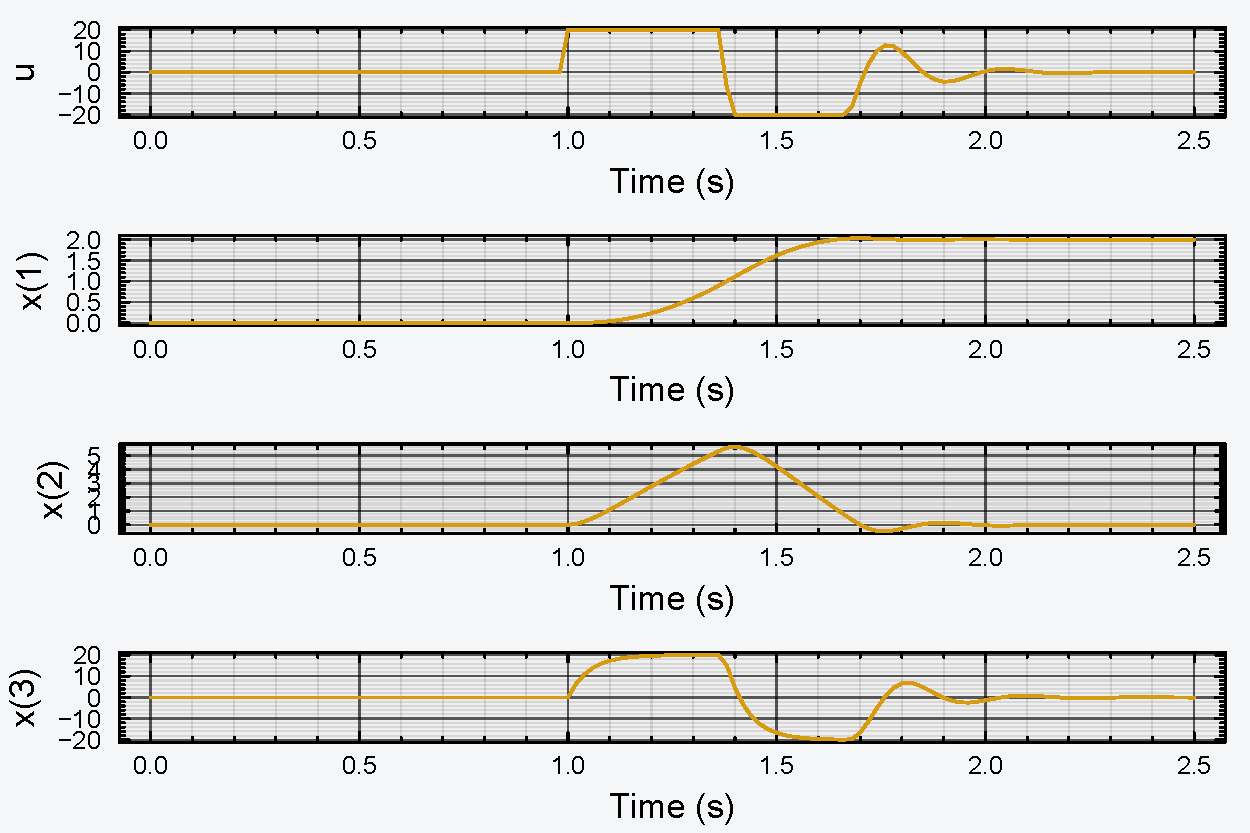
\includegraphics[keepaspectratio]{index_files/mediabag/block_on_slope/slope_files/figure-pdf/cell-7-output-1.pdf}}

For more stats:

\begin{Shaded}
\begin{Highlighting}[]
\NormalTok{si }\OperatorTok{=} \FunctionTok{stepinfo}\NormalTok{(res);}
\FunctionTok{plot}\NormalTok{(si);}\FunctionTok{title!}\NormalTok{(}\StringTok{"Step Response"}\NormalTok{)}
\end{Highlighting}
\end{Shaded}

\pandocbounded{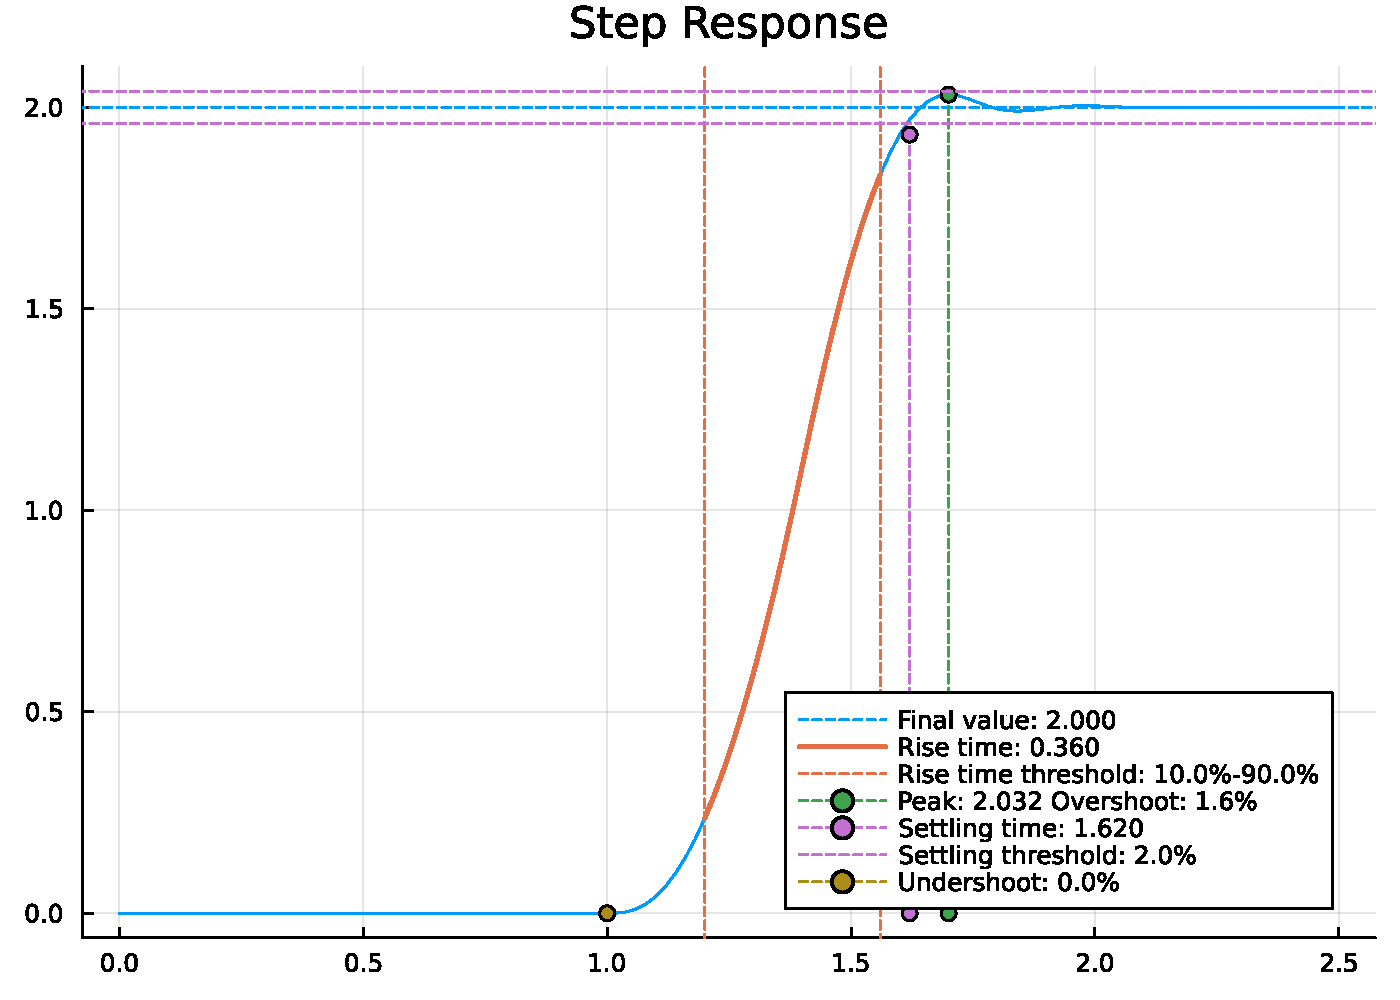
\includegraphics[keepaspectratio]{index_files/mediabag/block_on_slope/slope_files/figure-pdf/cell-8-output-1.pdf}}

We can also simulate it in a SIMULINK-like environment:

\begin{Shaded}
\begin{Highlighting}[]
\ImportTok{using} \BuiltInTok{FMI}\NormalTok{, }\BuiltInTok{DifferentialEquations}
\NormalTok{fmuPath }\OperatorTok{=} \FunctionTok{abspath}\NormalTok{(}\FunctionTok{joinpath}\NormalTok{(}\PreprocessorTok{@\_\_DIR\_\_}\NormalTok{,}
  \StringTok{".."}\NormalTok{,}\StringTok{".."}\NormalTok{,}
  \StringTok{"modelica"}\NormalTok{,}
  \StringTok{"ControlChallenges"}\NormalTok{,}
  \StringTok{"ControlChallenges.BlockOnSlope\_Challenges.Examples.WithFriction.fmu"}\NormalTok{))}
\NormalTok{fmu }\OperatorTok{=} \FunctionTok{loadFMU}\NormalTok{(fmuPath);}
\NormalTok{simData }\OperatorTok{=} \FunctionTok{simulateME}\NormalTok{(}
\NormalTok{    fmu,}
\NormalTok{    (}\FloatTok{0.0}\NormalTok{, }\FloatTok{5.0}\NormalTok{);}
\NormalTok{    recordValues}\OperatorTok{=}\NormalTok{[}\StringTok{"blockOnSlope.x"}\NormalTok{, }
    \StringTok{"blockOnSlope.xd"}\NormalTok{, }
    \StringTok{"blockOnSlope.usat"}\NormalTok{],}
\NormalTok{    showProgress}\OperatorTok{=}\ConstantTok{false}\NormalTok{);}
\FunctionTok{unloadFMU}\NormalTok{(fmu);}
\FunctionTok{plot}\NormalTok{(simData, states}\OperatorTok{=}\ConstantTok{false}\NormalTok{, timeEvents}\OperatorTok{=}\ConstantTok{false}\NormalTok{)}
\end{Highlighting}
\end{Shaded}

\pandocbounded{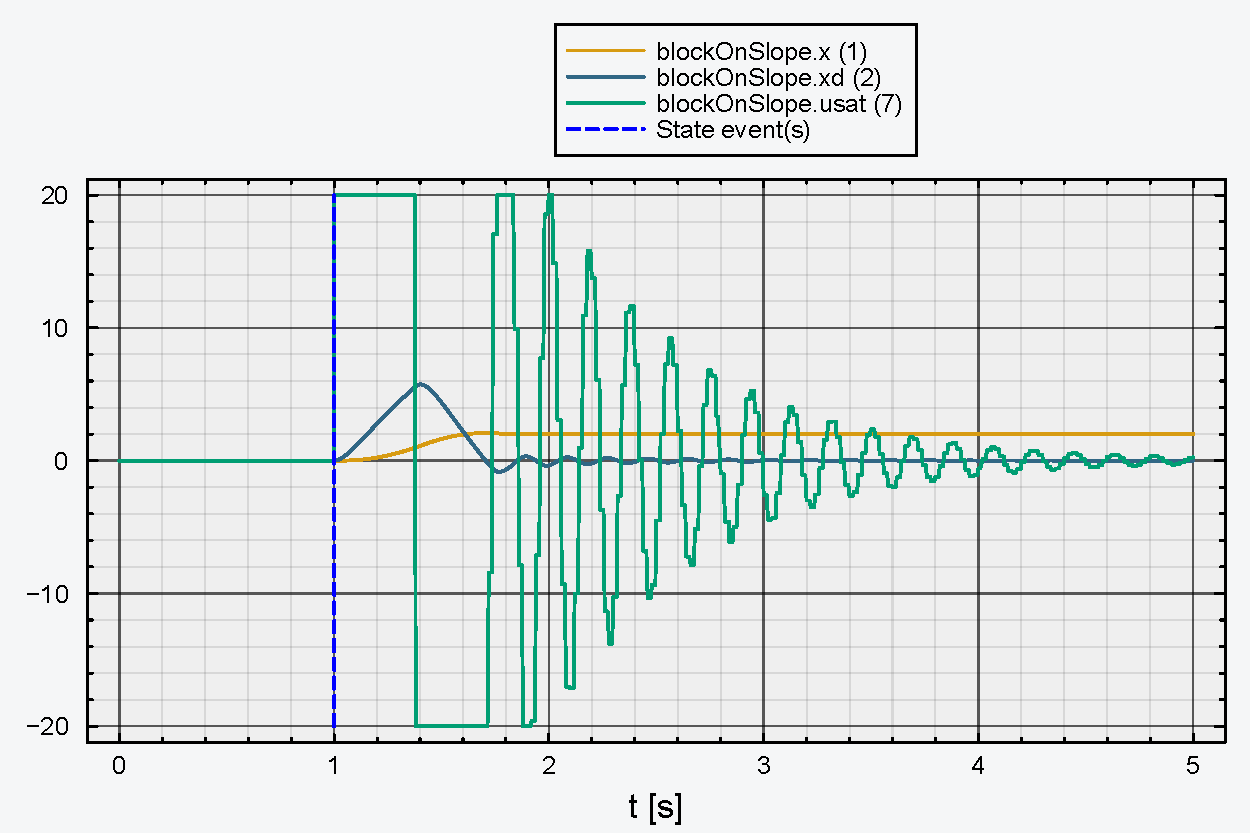
\includegraphics[keepaspectratio]{index_files/mediabag/block_on_slope/slope_files/figure-pdf/cell-9-output-1.pdf}}

There is a slight difference between the \texttt{lsim} simulation and
the FMU simulation. I need to recheck some stuff.



\cleardoublepage
\phantomsection
\addcontentsline{toc}{part}{Appendices}
\appendix

\chapter{Performance tricks}\label{performance-tricks}

\section{Hurwitz Check}\label{hurwitz-check}

Create our nice model. Assume to have run the \texttt{poles} function
and that you have a vector of eigenvalues. For simplicity I will create
an arbitrary vector with the first 100 values in \(-1\) and the last 100
values as random around \(0\).

\begin{Shaded}
\begin{Highlighting}[]
\ImportTok{using} \BuiltInTok{BenchmarkTools}

\NormalTok{vbig }\OperatorTok{=}\NormalTok{ [}\FunctionTok{zeros}\NormalTok{(}\DataTypeTok{ComplexF64}\NormalTok{,}\FloatTok{100}\NormalTok{)}\OperatorTok{.{-}}\FloatTok{1}\NormalTok{ ; }\FunctionTok{rand}\NormalTok{(}\DataTypeTok{ComplexF64}\NormalTok{,}\FloatTok{100}\NormalTok{)}\OperatorTok{.{-}}\FloatTok{0.5}\NormalTok{];}

\NormalTok{vbig[[}\FloatTok{1}\NormalTok{,}\KeywordTok{end}\NormalTok{]]}
\end{Highlighting}
\end{Shaded}

\begin{verbatim}
2-element Vector{ComplexF64}:
                  -1.0 + 0.0im
 -0.030437584033531584 + 0.17283801604223903im
\end{verbatim}

\subsection{\texorpdfstring{\texttt{for}
loop}{for loop}}\label{for-loop}

With a naive approach we check if all the elements are in the LHP: make
a function that iterates and returns false if it hits a pole with
positive real part.

\begin{Shaded}
\begin{Highlighting}[]
\KeywordTok{function} \FunctionTok{isHurwitz}\NormalTok{(v)}
    \ControlFlowTok{for}\NormalTok{ i }\KeywordTok{in} \FunctionTok{eachindex}\NormalTok{(v)}
        \ControlFlowTok{if} \FunctionTok{real}\NormalTok{(v[i])}\OperatorTok{\textgreater{}}\FloatTok{0.0}
            \ControlFlowTok{return} \ConstantTok{false}
        \ControlFlowTok{end}
    \ControlFlowTok{end}
    \ControlFlowTok{return} \ConstantTok{true}
\KeywordTok{end}

\PreprocessorTok{@benchmark} \FunctionTok{isHurwitz}\NormalTok{(}\OperatorTok{$}\NormalTok{(}\FunctionTok{Ref}\NormalTok{(vbig))[])}
\end{Highlighting}
\end{Shaded}

\begin{verbatim}
BenchmarkTools.Trial: 10000 samples with 987 evaluations per sample.
 Range (min … max):  49.949 ns … 969.301 ns  ┊ GC (min … max): 0.00% … 0.00%
 Time  (median):     54.306 ns               ┊ GC (median):    0.00%
 Time  (mean ± σ):   57.041 ns ±  22.237 ns  ┊ GC (mean ± σ):  0.00% ± 0.00%

  ▆▇▆█▇▅▄▃▂▂▁▁▁▁                                               ▂
  ██████████████▇█▇▇▆▆▆▆▇▆▆▅▅▅▆▅▆▄▄▅▄▅▅▅▅▅▅▄▄▅▄▁▅▃▃▄▄▆▇▁▁▅▆▇▆▆ █
  49.9 ns       Histogram: log(frequency) by time       126 ns <

 Memory estimate: 0 bytes, allocs estimate: 0.
\end{verbatim}

We have our baseline. We can probably squeeze out some more performance
but I'm still a Julia noob.

\subsection{\texorpdfstring{\texttt{all()}}{all()}}\label{all}

Let's try using some of the built-in declarative functions:

\begin{Shaded}
\begin{Highlighting}[]
\PreprocessorTok{@benchmark} \FunctionTok{all}\NormalTok{(}\FunctionTok{real}\NormalTok{(}\OperatorTok{$}\NormalTok{vbig)}\OperatorTok{.\textless{}=}\FloatTok{0.0}\NormalTok{)}
\end{Highlighting}
\end{Shaded}

\begin{verbatim}
BenchmarkTools.Trial: 10000 samples with 746 evaluations per sample.
 Range (min … max):  183.378 ns …  22.068 μs  ┊ GC (min … max):  0.00% … 97.78%
 Time  (median):     261.662 ns               ┊ GC (median):     0.00%
 Time  (mean ± σ):   445.850 ns ± 864.436 ns  ┊ GC (mean ± σ):  32.85% ± 16.78%

  █▇▅▃▁▁▁▁                                                      ▂
  ██████████▇▆▅▅▅▄▄▅▃▃▁▁▁▁▁▃▅▆▅▅▃▃▃▄▃▃▄▄▃▄▅▆▇▇▇▇▇▆▅▆▅▆▅▅▅▅▅▅▅▅▆ █
  183 ns        Histogram: log(frequency) by time        5.1 μs <

 Memory estimate: 1.75 KiB, allocs estimate: 5.
\end{verbatim}

Simple \texttt{all()}, when given a tuple it checks if all the values
are \texttt{True}, otherwise it stops when it encounters the first
\texttt{False}.

We can see that it's a tad slower. This is because it's creating a new
vector with just the real parts, then it's creating a new vector with
only the boolean results and then it's checking if there are any False
results.

This results in a lot of allocations and wasted resources.

\begin{Shaded}
\begin{Highlighting}[]
\PreprocessorTok{@benchmark} \FunctionTok{all}\NormalTok{(}\OperatorTok{\textless{}=}\NormalTok{(}\FloatTok{0.0}\NormalTok{),}\FunctionTok{real}\NormalTok{(}\OperatorTok{$}\NormalTok{vbig))}
\end{Highlighting}
\end{Shaded}

\begin{verbatim}
BenchmarkTools.Trial: 10000 samples with 759 evaluations per sample.
 Range (min … max):  144.664 ns …  31.398 μs  ┊ GC (min … max):  0.00% … 97.98%
 Time  (median):     226.746 ns               ┊ GC (median):     0.00%
 Time  (mean ± σ):   344.335 ns ± 699.060 ns  ┊ GC (mean ± σ):  22.41% ± 15.26%

  ▂██▆▃▂▁       ▁▂▁▁▁                                           ▂
  ████████▇▇▆▅▇███████▇▇▇▆▅▅▃▄▄▄▁▄▃▃▃▁▁▄▃▃▃▁▁▁▁▁▁▁▁▃▄▆▆▇███▇▆▇▆ █
  145 ns        Histogram: log(frequency) by time       2.44 μs <

 Memory estimate: 1.62 KiB, allocs estimate: 2.
\end{verbatim}

A smarter way is to skip on of the allocations by creating the vector of
real parts and then checking row by row if the non-positivity check
fails.

\begin{Shaded}
\begin{Highlighting}[]
\PreprocessorTok{@benchmark} \FunctionTok{all}\NormalTok{(i }\OperatorTok{{-}\textgreater{}} \FunctionTok{real}\NormalTok{(i)}\OperatorTok{\textless{}=}\FloatTok{0.0}\NormalTok{,}\OperatorTok{$}\NormalTok{vbig)}
\end{Highlighting}
\end{Shaded}

\begin{verbatim}
BenchmarkTools.Trial: 10000 samples with 987 evaluations per sample.
 Range (min … max):  49.139 ns …  2.022 μs  ┊ GC (min … max): 0.00% … 0.00%
 Time  (median):     51.773 ns              ┊ GC (median):    0.00%
 Time  (mean ± σ):   53.295 ns ± 22.061 ns  ┊ GC (mean ± σ):  0.00% ± 0.00%

  ▅▆█▃▂▂                                                      ▁
  ███████▇▅▆▆▅▄▅▃▄▄▁▅▅▅▄▃▄▅▄▄▄▁▃▃▃▅▁▄▃▄▃▃▃▄▁▄▃▃▃▃▃▁▃▃▃▃▃▄▄▃▁█ █
  49.1 ns      Histogram: log(frequency) by time       116 ns <

 Memory estimate: 0 bytes, allocs estimate: 0.
\end{verbatim}

We can do better: Instead of converting into real the full vector it
checks element by element if it's in the LHP. It returns false at the
first failure. We finally have a comparable result to the benchmark
function but in a more compact way.

Is it cleaner? That's subjective.

\subsection{\texorpdfstring{\texttt{mapreduce()}}{mapreduce()}}\label{mapreduce}

Finally we try the MapReduce approach. This allows a better utilization
of your processor without the necessity of learning parallel
programming.

\begin{Shaded}
\begin{Highlighting}[]
\PreprocessorTok{@benchmark} \FunctionTok{mapreduce}\NormalTok{(}\FunctionTok{i{-}\textgreater{}real}\NormalTok{(i)}\OperatorTok{\textless{}=}\FloatTok{0.0}\NormalTok{, }\OperatorTok{\&}\NormalTok{, }\OperatorTok{$}\NormalTok{vbig)}
\end{Highlighting}
\end{Shaded}

\begin{verbatim}
BenchmarkTools.Trial: 10000 samples with 993 evaluations per sample.
 Range (min … max):  42.095 ns … 692.346 ns  ┊ GC (min … max): 0.00% … 0.00%
 Time  (median):     43.807 ns               ┊ GC (median):    0.00%
 Time  (mean ± σ):   46.318 ns ±  15.245 ns  ┊ GC (mean ± σ):  0.00% ± 0.00%

  ▇█▆▄▅▄▂▁ ▁  ▁                                                ▂
  █████████████▆▆▆▆▅▇▆█▆▆▅▄▅▄▄▃▆▆▃▁▄▅▅▁▃▄▃▁▄▄▄▃▄▄▅▆▃▄▃▄▄▅▇▆▇▆▆ █
  42.1 ns       Histogram: log(frequency) by time       102 ns <

 Memory estimate: 0 bytes, allocs estimate: 0.
\end{verbatim}

We squeeze the last bit of performance and beat the initial benchmark,
not by much but still appreciable.




\end{document}
